\documentclass{article}

\usepackage[utf8]{inputenc}
\usepackage[french]{babel}

\usepackage{lmodern}
\usepackage{graphicx}
\usepackage{hyperref}
\usepackage{graphicx}
\usepackage{natbib}
\usepackage{tcolorbox}
\usepackage{xcolor}
\usepackage{array}
\usepackage{pifont}
\usepackage[a4paper, margin=1.5cm]{geometry}  
\usepackage{longtable}
\usepackage{float}

\graphicspath{ {./res/} }

\definecolor{needcolor}{HTML}{007ACC}
\definecolor{nonfunctionnalneedcolor}{HTML}{9722ff}
\definecolor{subneedcolor}{HTML}{28A745}
\definecolor{duedateassigncolor}{HTML}{FF9800}

\tcbuselibrary{skins, breakable}
\newtcolorbox{needbox}[1][]{
  colframe=needcolor,
  colback=needcolor!10,
  coltitle=white,
  fonttitle=\bfseries,
  title=#1,
  breakable,
  enhanced,
  sharp corners=all
}

\newtcolorbox{nonfunctionnalneedbox}[1][]{
  colframe=nonfunctionnalneedcolor,
  colback=nonfunctionnalneedcolor!10,
  coltitle=white,
  fonttitle=\bfseries,
  title=#1,
  breakable,
  enhanced,
  sharp corners=all
}

\newtcolorbox{justificationbox}[1][]{
  colframe=subneedcolor,
  colback=subneedcolor!10,
  coltitle=white,
  fonttitle=\bfseries,
  title=#1,
  breakable,
  enhanced,
  sharp corners=all
}

\newcommand{\valid}{\textcolor{green}{\ding{108}}}  % Cercle vert pour validé
\newcommand{\semivalid}{\textcolor{orange}{\ding{108}}}  % Cercle orange pour semi-validé
\newcommand{\nonvalid}{\textcolor{red}{\ding{108}}}  % Cercle rouge pour non-validé

\author{
    Valentin Jonquière,
    Mathilde Chollon,
    Denis Demirci,
    Iwen Jomaa,
    Jonathan Landry
}

\title{Rapport Final projet de programmation, Échecs en Java}

\begin{document}

\maketitle

\pagebreak

\tableofcontents

\pagebreak
\begin{abstract}
    Ce rapport synthétise le travail réalisé lors de l'UE Projet de Programmation de Master 1 Informatique à l'Université de Bordeaux.
 \end{abstract}

\section{Description de l'existant}
\subsection{Origine des Échecs}
Le jeu d’échecs, aussi appelé le jeu des Rois, est un jeu de stratégie dans lequel deux joueurs s’affrontent,
et le but est de faire échec et mat, c’est-à-dire arriver dans une position où il est possible de capturer
le Roi adverse et donc gagner la partie après n’importe quel coup joué par notre opposant (hormis capturer notre roi).
Le jeu d’échecs se joue sur un échiquier, un plateau de 8 lignes et 8 colonnes, 64 cases au total avec des pièces
caractérisées par certaines propriétés uniques. De manière compétitive, le jeu d'échecs effectue un classement
basé sur un système de points, appelés "Élos". Il sert à estimer le niveau d'un joueur (humain comme ordinateur) et
à répartir ces joueurs en catégories. Pour donner un ordre d'idée, le champion du monde possède un Élo aux alentours de 2900,
tandis qu'un joueur débutant qui connaît comment les pièces se déplacent est aux alentours des 400 Élos. Ce système d'Élo
va notamment nous permettre d'approximer le niveau de notre Intelligence Artificielle développée dans le cadre de ce projet.\\
Les origines de ce jeu restent méconnues, mais la légende la plus célèbre raconte que le précepteur d’un jeune prince en Inde
voulait simplifier les mécanismes de la société et inventa ainsi un échiquier avec des pièces, chacune jouant un rôle précis,
avec le Roi, la pièce maîtresse. Le prince fut alors émerveillé et en gage de remerciements, il demanda à son précepteur ce
qu’il souhaitait avoir comme présent. Ce dernier répondit qu’il voulait 1 grain de riz sur la première case, 2 grains de riz
sur la deuxième, 4 grains de riz sur la troisième, etc. jusqu’à la dernière case. Sur la 64ème case, il avait donc
2 puissance 63 grains de riz, soit de quoi recouvrir le pays entier avec une couche de riz.

\subsection{Variantes du jeu d'échecs}
À travers les années, les échecs ont été popularisés et ont donné naissance à de nombreuses variantes. Parmi les plus connues, on trouve :
\begin{itemize}
    \item Les échecs aléatoires de Fischer (Chess960) : Une variante inventée en 1996 par Bobby Fischer où la position initiale des pièces est aléatoire
    (mais reste miroir, c'est-à-dire que les blancs et les noirs commencent avec la même position). Ce mode favorise la créativité au détriment de la mémorisation des ouvertures.
    \item Les échecs Capablanca : Une version jouée sur un échiquier plus grand (10x8 ou 10x10) avec des pièces supplémentaires comme l'archer et le chancelier. Cette variante a été inventée en 1984 par le créateur de jeux hollandais Christian Freeling.
    \item Les échecs japonais : Le Shôgi, où contrairement aux échecs occidentaux, la partie se termine dès que le roi est capturé, ou lorsque l'un
    des deux joueurs abandonne. Il n'y a pas d'échec et mat à proprement parler. Les origines de cette variante asiatique reste inconnue,
    mais des rumeurs disent qu'ils ont été inspirés des échecs chinois, à l'époque de Nara (710-794).
\end{itemize}
Notre projet concerne les échecs classiques, ou traditionnels. On peut considérer que l'on admet une variation: celle du Blitz, si ce mode
est vu comme une variante.

\subsection{Moments clés dans l’histoire des échecs}
Le jeu d’échecs a été animé par des confrontations historiques et importantes. Notamment deux très connues que voici :
\begin{itemize}
    \item Fischer vs. Spassky (1972) : Ce duel de la Guerre Froide a opposé l’Américain Bobby Fischer au Soviétique
    Boris Spassky. Fischer a remporté le championnat du monde, mettant fin à l'interminable domination des soviétiques
    aux échecs. Les États-Unis ressortent ainsi victorieux face à l'URSS.
    \item Kasparov vs. Karpov (1984-1985) : Un des matchs les plus longs de l’histoire, où Anatoli Karpov et Garry Kasparov
    se sont affrontés pendant des mois avant que le match soit interrompu sans vainqueur, puis rejoué et remporté par Kasparov.
    \item Kasparov vs. Deep Blue (1997) : Ce fut la première victoire d'un ordinateur contre un champion du monde des échecs en match officiel.
    Cette date marque notamment l'ascension de l'Intelligence Artificielle dans le monde des échecs.
\end{itemize}
Ces événements ont façonné l’histoire du jeu. La perception des échecs dans la culture populaire a changé et de nombreuses
personnes se sont mises à jouer.

\subsection{L’évolution des chess engines}
L’intelligence artificielle a pris une place très importante dans le jeu d'échecs, à tel point que les échecs
sont analysés et perçus d'une autre manière. Parmi les avancées majeures, on retrouve :
\begin{itemize}
    \item Deep Blue : Programme célèbre pour avoir battu Garry Kasparov en 1997. Ce programme était exécuté par des super-calculateurs
    de l'époque, avec 32 coeurs, 256 threads au total.
    \item Stockfish : Engine open-source extrêmement puissant, probablement le meilleur aujourd'hui, basé sur notamment une évaluation positionnelle
    grâce à des heuristiques avancées et des optimisations algorithmiques.
    \item Leela Chess Zero (Lc0) : Engine particulièrement connu pour utiliser un réseau de neurones basé sur le deep learning, inspiré du fameux
    modèle AlphaZero de Google DeepMind.
\end{itemize}
Ces chess engines sont aujourd’hui utilisés pour analyser des parties, préparer des parties, et même aider les
joueurs humains à progresser. Au jeu d'échecs, l'Intelligence Artificielle est notamment connue pour être très agressive
(en terme de stratégie de jeu). Cela fait maintenant presque 30 ans qu'il impossible pour un humain de gagner contre
le meilleur ordinateur aux échecs (autour des 3600 Élos aujourd'hui, environ 2900 pour Deep Blue en 1997).

Les échecs étant un jeu universel, ils ont été étudiés et un grand nombre de papiers scientifiques
sont disponibles. Ceux-ci nous seront très utiles tout au long du projet, car ils concernent des
besoins différents. Tout d'abord une grande partie des papiers que nous allons utiliser sont en rapport
avec la partie intelligence artificielle du développement. C'est pour cela que nous avons par exemple
choisi de nous baser sur l'article `Programming a computer for playing chess' \cite{Shannon1950}, 
puisqu'il possède une partie consacrée à la construction d'heuristiques efficace pour les échecs.
Nous avons également basé nos recherches sur la thèse `Using Monte Carlo Tree Search to play chess' \cite{Kral2021}
de Jakub Král sur l'utlisation de différents algorithmes au service des échecs, tels que AlphaBeta ou
Monte Carlo Tree Seach. Pour la partie intelligence artificielle, nous avons choisi de nous baser sur le 
`Zobrist hashing' \cite{ZobristHashing} afin de ne pas réévaluer des positions déjà évaluées lors de la 
recherche du meilleur coup à jouer par le joueur artificiel \ref{Zobrist}. Nous avons également orienté
nos recherches sur la représentation du jeu d'échecs par les bitmaps (plateau, représentation des coups) \cite{Bijl2021}.
Pour finir, nous avons utilisé un papier plus général, mais contenant des informations sur le développement
d'un moteur d'échecs en java \cite{PaulDailly}. Nous nous servons également des deux articles présents sur 
notre repository Gitlab, \cite{Bitboards} et \cite{GameBitboards}, qui concernent aussi les Bitboards.

\section{Règles du jeu}
Le jeu d'échecs contient beaucoup de règles, parfois techniques, mais dont l'objectif reste simple à comprendre :
il faut mettre le roi adverse en \textbf{échec et mat} pour gagner la partie. Cela signifie que le roi est en \textbf{échec},
mais n'a aucun coup légal pour se défendre de cette attaque. Il faut différencier la règle \textbf{échec} et 
\textbf{échec et mat}. Un Roi qui est en situation d'\textbf{échec} est un Roi qui est attaqué par une pièce
ennemie, mais qui peut se défendre pour sortir de cette situation (car en tant que joueur, on ne doit pas capturer notre Roi,
la pièce maîtresse). Donc finalement, être en \textbf{échecs et mat} signifie être en \textbf{échec}, mais sans avoir
la possibilité de se défendre, c'est-à-dire que le Roi est capturé par l'adversaire après n'importe quel coup joué.

\subsection{L'échiquier et les pièces}
Les échecs se jouent sur un échiquier de 64 cases disposé en 8x8. Chaque joueur commence la partie avec 16 pièces :
\begin{itemize}
    \item 1 roi
    \item 1 dame
    \item 2 tours
    \item 2 cavaliers
    \item 2 fous
    \item 8 pions
\end{itemize}

\begin{figure}[h]
    \centering
    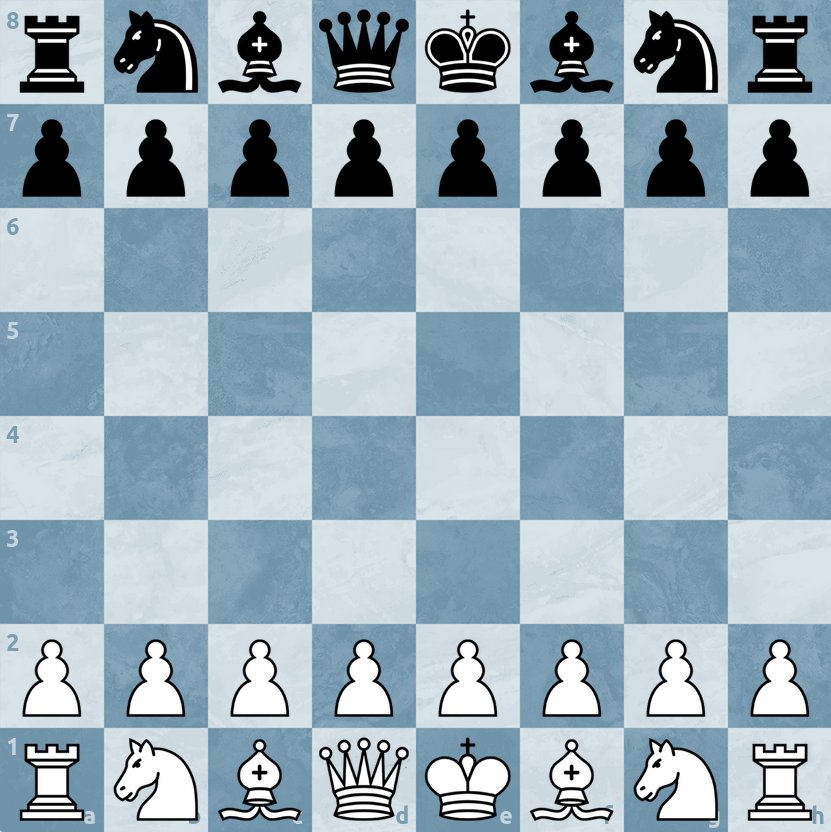
\includegraphics[width=\textwidth,height=5.0cm,keepaspectratio]{jeuDepart.png}
    \caption{Position initiale des pièces}
\end{figure}

Le joueur avec les pièces blanches commence. Ensuite, chaque joueur joue à tour de rôle, un déplacement de pièce par tour.

\subsection{Déplacements des pièces}

Les déplacements sont propres à chaque type de pièce :

\subsubsection*{Pion}
Le pion avance uniquement en ligne droite, d'une case à la fois. Lors de son premier déplacement, il peut avancer de deux cases. Il capture les pièces adverses en diagonale.

\begin{figure}[h]
    \centering
    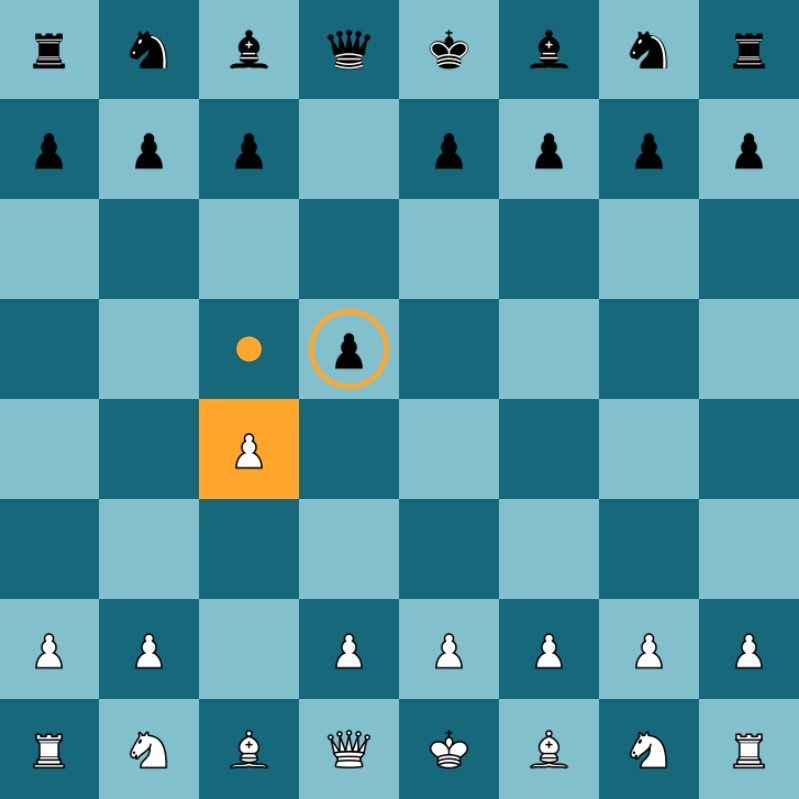
\includegraphics[width=\textwidth,height=5.0cm,keepaspectratio]{pionMove.png}
    \caption{Déplacement du pion}
\end{figure}

\subsubsection*{Cavalier}
Le cavalier se déplace en forme de "L" : deux cases dans une direction, puis une case perpendiculaire. Il peut sauter par-dessus d'autres pièces.

\begin{figure}[h]
    \centering
    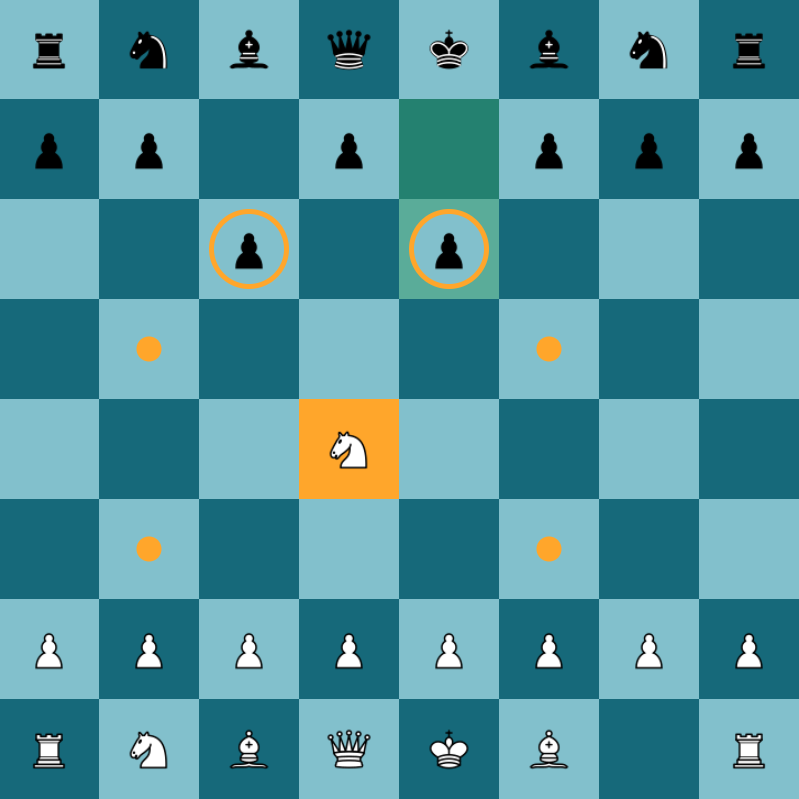
\includegraphics[width=\textwidth,height=5.0cm,keepaspectratio]{cavalierMove.png}
    \caption{Déplacement du cavalier}
\end{figure}

\subsubsection*{Fou}
Le fou se déplace en diagonale sur un nombre illimité de cases, sans sauter d'autres pièces. Il reste toujours sur des cases de la même couleur.

\begin{figure}[h]
    \centering
    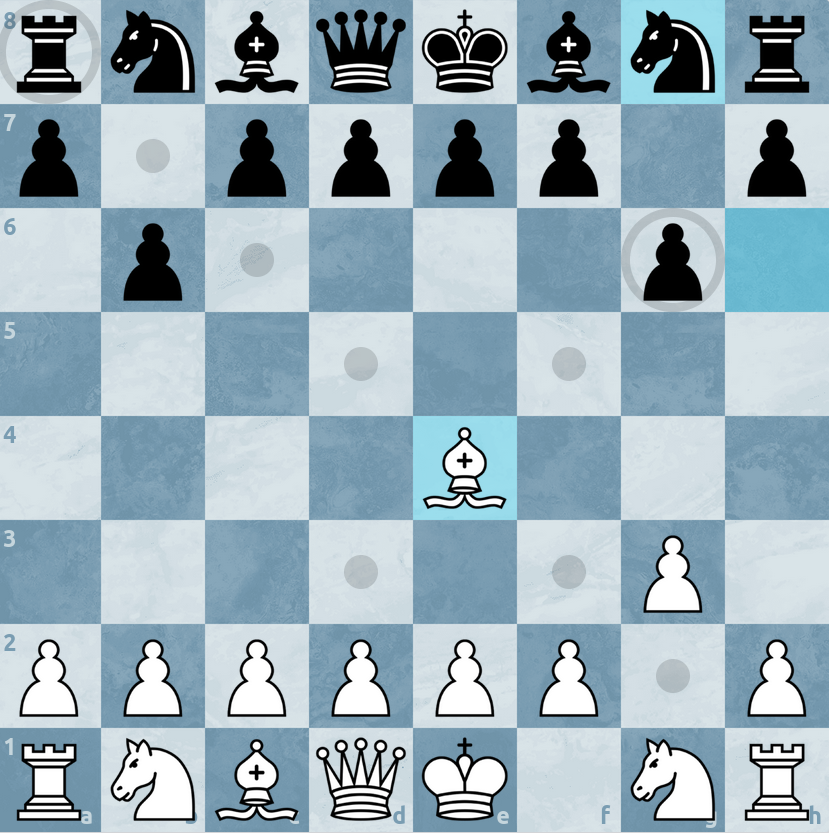
\includegraphics[width=\textwidth,height=5.0cm,keepaspectratio]{fouMove.png}
    \caption{Déplacement du fou}
\end{figure}

\subsubsection*{Tour}
La tour se déplace horizontalement ou verticalement sur un nombre illimité de cases. Elle contrôle des lignes entières.

\begin{figure}[h]
    \centering
    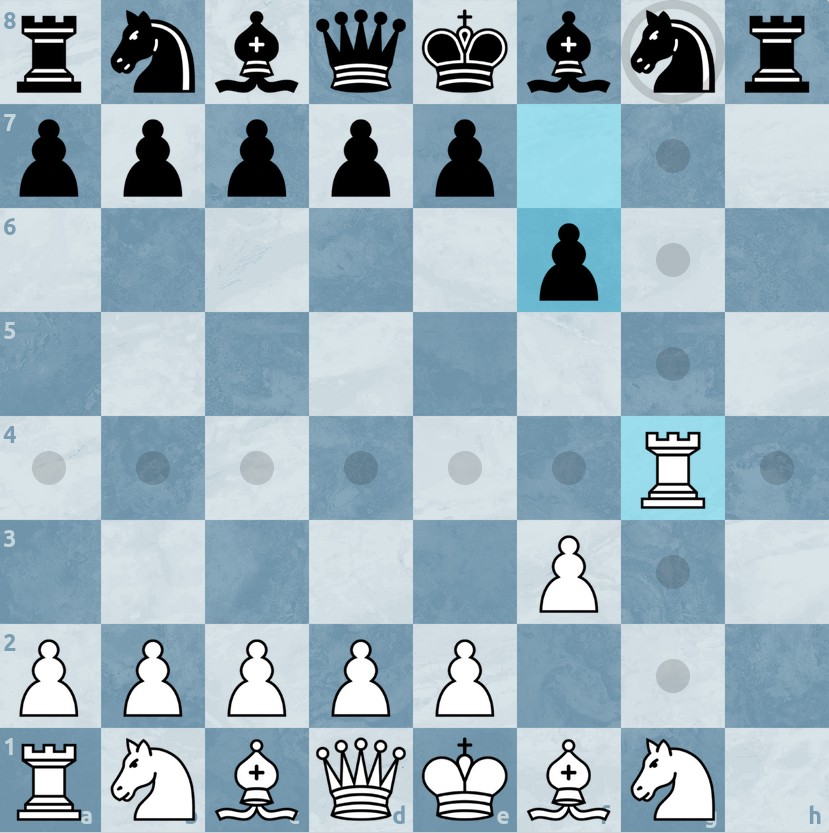
\includegraphics[width=\textwidth,height=5.0cm,keepaspectratio]{tourMove.png}
    \caption{Déplacement de la tour}
\end{figure}

\subsubsection*{Dame}
La dame combine les mouvements du fou et de la tour. Elle peut se déplacer horizontalement, verticalement et en diagonale.

\begin{figure}[h]
    \centering
    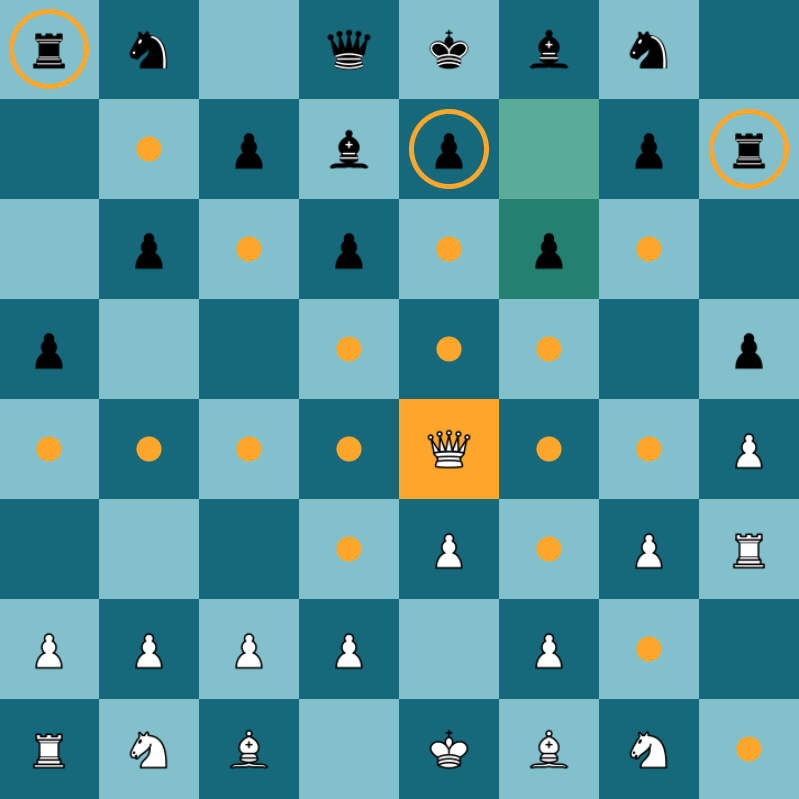
\includegraphics[width=\textwidth,height=5.0cm,keepaspectratio]{dameMove.png}
    \caption{Déplacement de la dame}
\end{figure}

\subsubsection*{Roi}
Le roi se déplace d'une case dans toutes les directions. Il est la pièce la plus importante, mais aussi vulnérable.

\begin{figure}[h]
    \centering
    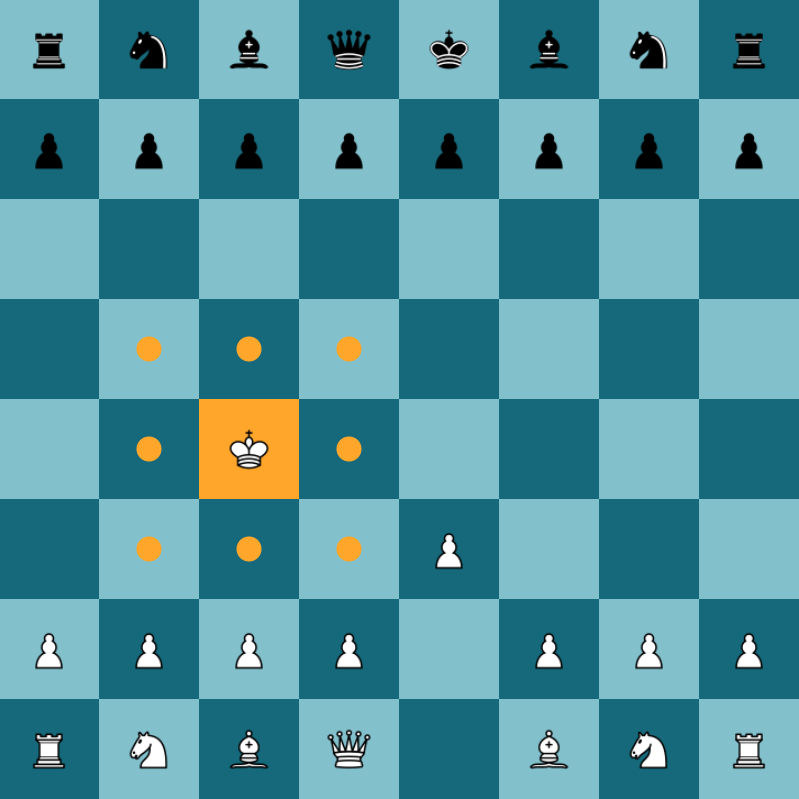
\includegraphics[width=\textwidth,height=5.0cm,keepaspectratio]{roiMove.png}
    \caption{Déplacement du roi}
\end{figure}

\subsection{Règles spécifiques}

\subsubsection*{Clouage}
Lorsqu'une pièce intercepte une menace dirigée contre le roi, elle est \textbf{clouée} : elle ne peut pas bouger, sous peine de mettre le roi en échec.

\begin{figure}[h]
    \centering
    \begin{minipage}[b]{0.45\textwidth}
        \centering
        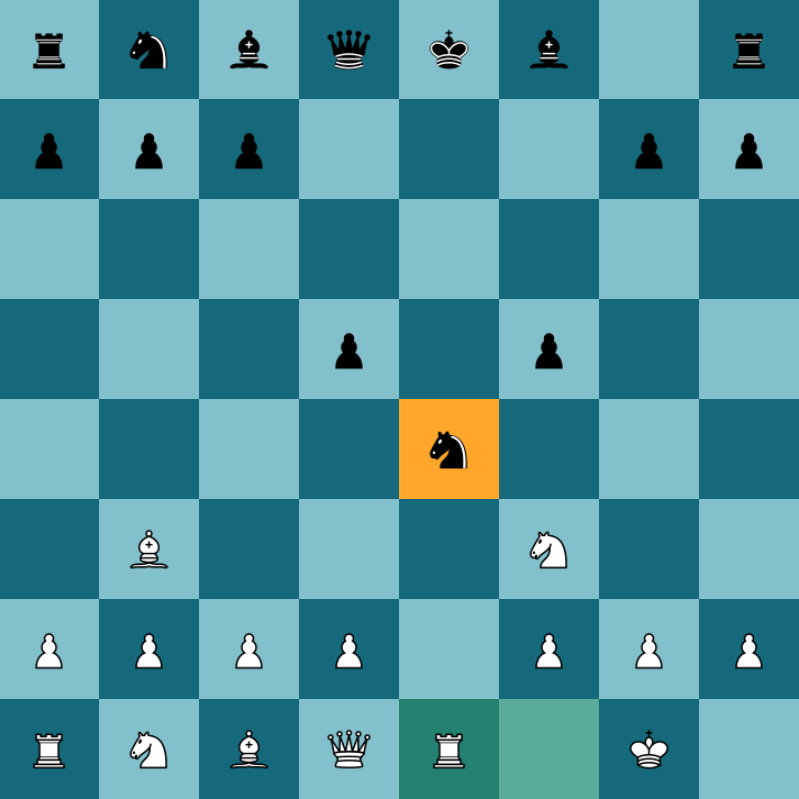
\includegraphics[width=\textwidth,height=5cm,keepaspectratio]{clouage1.png}
    \end{minipage}
    \hspace{0.005\textwidth}
    \begin{minipage}[b]{0.45\textwidth}
        \centering
        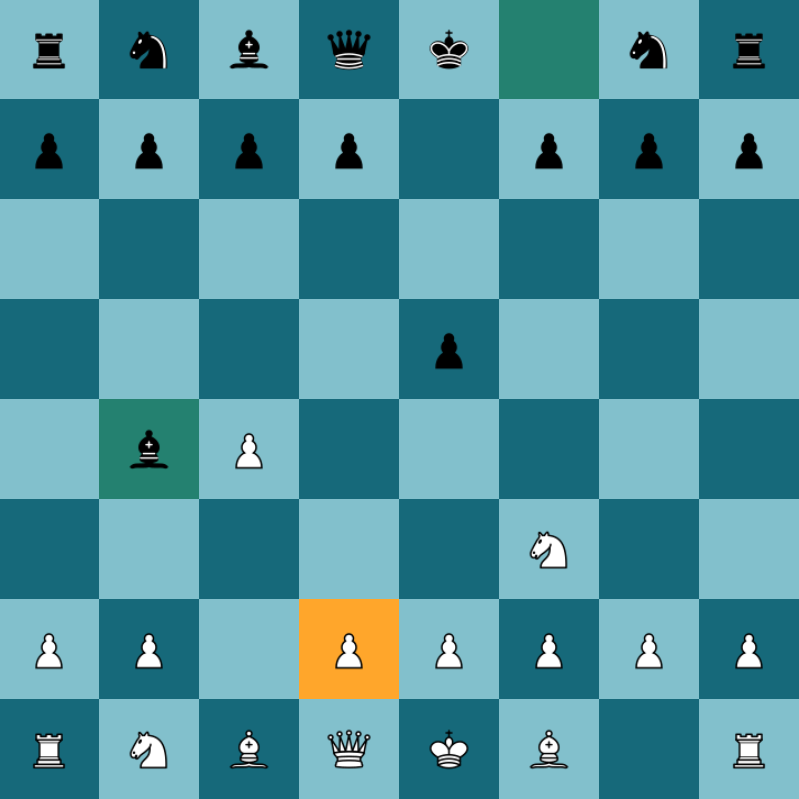
\includegraphics[width=\textwidth,height=5cm,keepaspectratio]{clouage2.png}
    \end{minipage}
    \caption{Exemple de Clouage}
\end{figure}

\subsubsection*{Roque}
Le \textbf{roque} est un mouvement spécial impliquant le roi et une tour. Il est soumis aux conditions suivantes :
\begin{itemize}
    \item Ni le roi ni la tour n'ont bougé.
    \item Le roi n'est pas en échec.
    \item Aucune des cases traversées par le roi n'est attaquée.
    \item Aucune pièce ne se trouve entre le roi et la tour.
\end{itemize}

\begin{figure}[h]
    \centering
    \begin{minipage}[b]{0.45\textwidth}
        \centering
        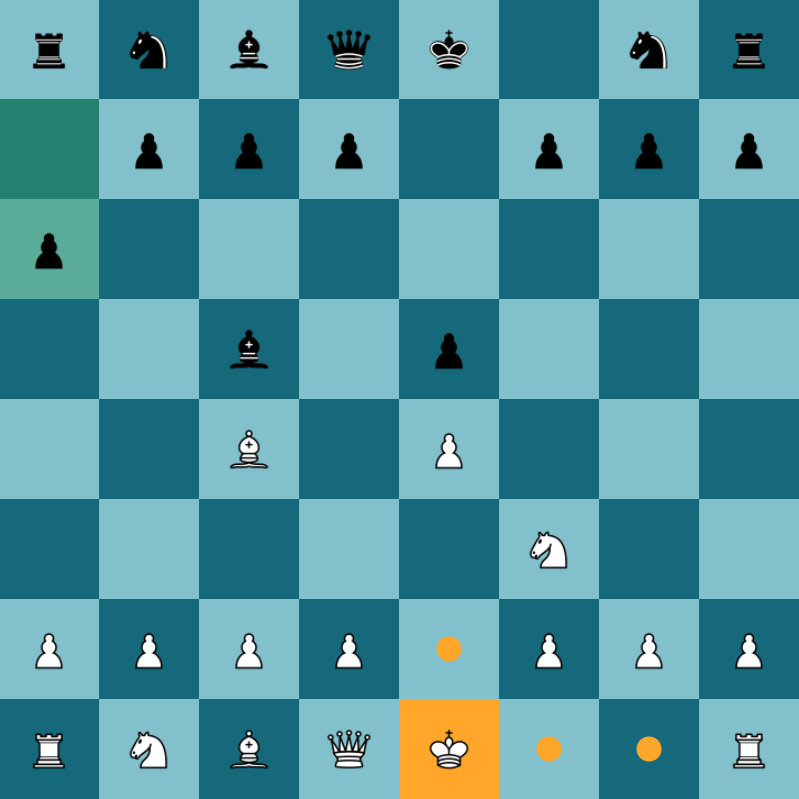
\includegraphics[width=\textwidth,height=5cm,keepaspectratio]{roque1.png}
    \end{minipage}
    \hspace{0.005\textwidth}
    \begin{minipage}[b]{0.45\textwidth}
        \centering
        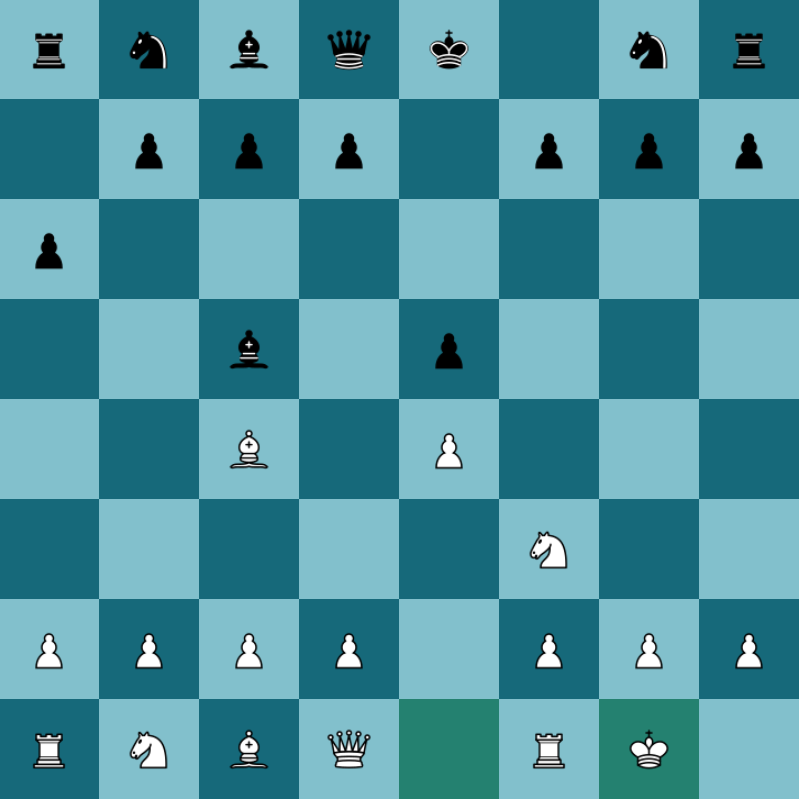
\includegraphics[width=\textwidth,height=5cm,keepaspectratio]{roque2.png}
    \end{minipage}
    \caption{Exemple de Roque}
\end{figure}

\subsubsection*{Prise en passant}
Lorsqu'un pion adverse avance de deux cases depuis sa position initiale et finit à côté de l’un de nos pions, on peut le capturer \textbf{en passant} au coup suivant uniquement.

\begin{figure}[H]
    \centering
    \begin{minipage}[b]{0.45\textwidth}
        \centering
        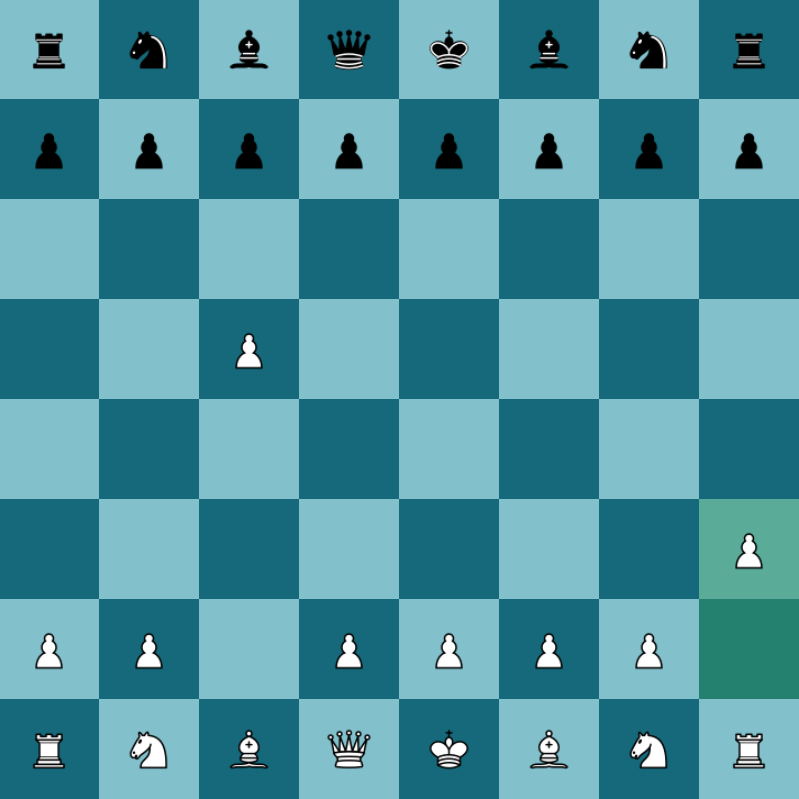
\includegraphics[width=\textwidth,height=5cm,keepaspectratio]{enpassant1.png}
    \end{minipage}
    \hspace{0.005\textwidth}
    \begin{minipage}[b]{0.45\textwidth}
        \centering
        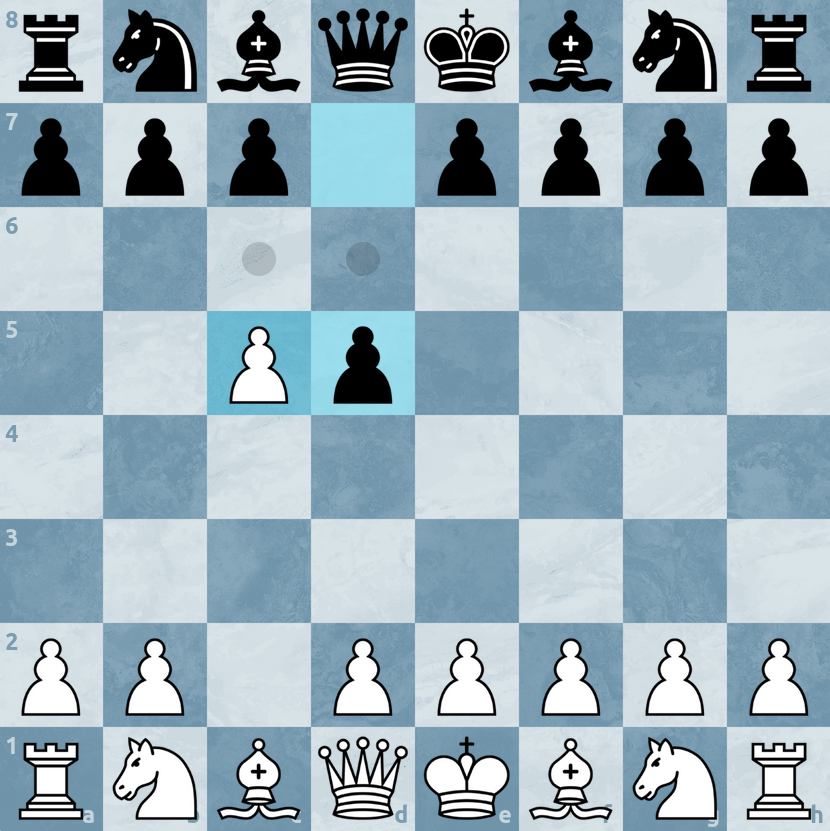
\includegraphics[width=\textwidth,height=5cm,keepaspectratio]{enpassant2.png}
    \end{minipage}
    \caption{Exemple d'En passant}
\end{figure}

\subsubsection*{Promotion du pion}
Lorsqu'un pion atteint la dernière rangée, il peut être promu en dame, tour, fou ou cavalier. Cette promotion peut représenter un avantage décisif.

\begin{figure}[H]
    \centering
    \begin{minipage}[b]{0.45\textwidth}
        \centering
        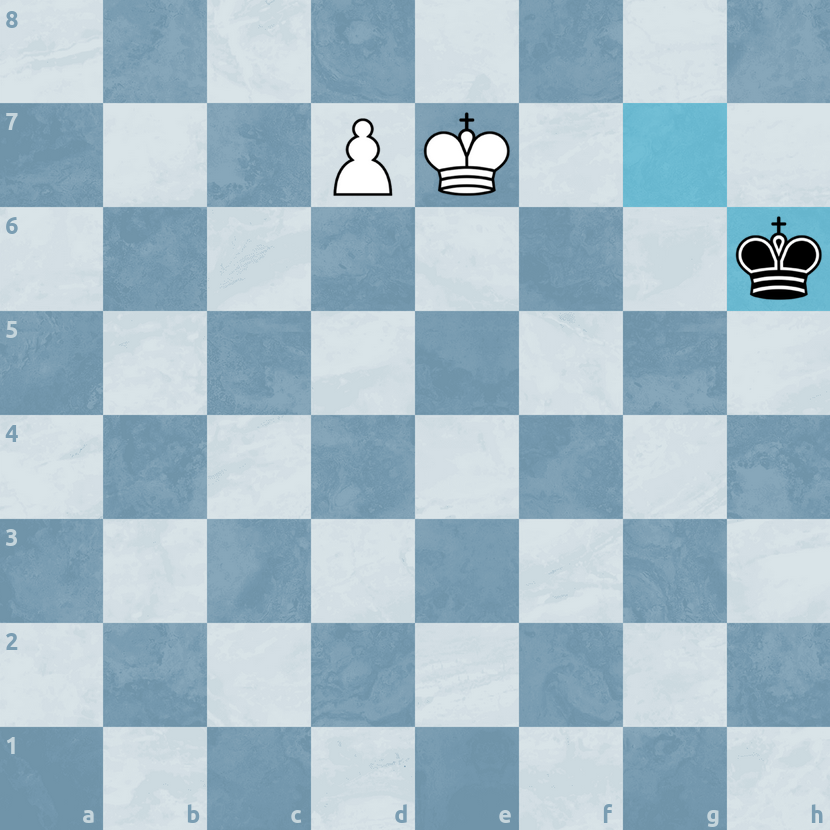
\includegraphics[width=\textwidth,height=5cm,keepaspectratio]{promotion1.png}
    \end{minipage}
    \hspace{0.005\textwidth}
    \begin{minipage}[b]{0.45\textwidth}
        \centering
        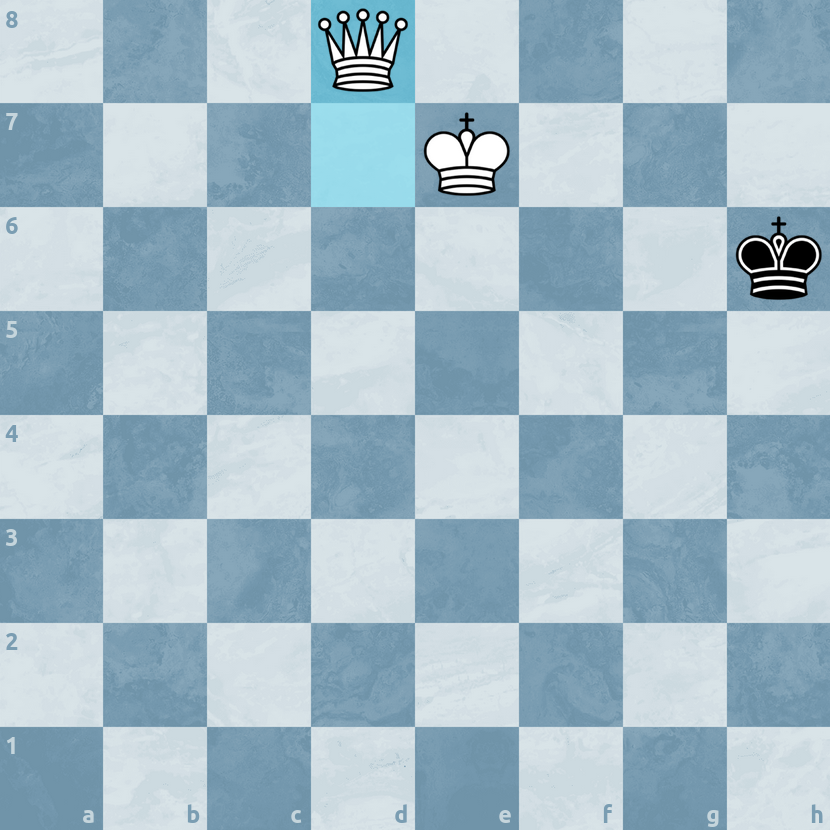
\includegraphics[width=\textwidth,height=5cm,keepaspectratio]{promotion2.png}
    \end{minipage}
    \caption{Exemple de promotion}
\end{figure}

\subsection{Fin de Partie}
Une partie d'échecs peut se terminer de plusieurs façons :
\begin{itemize}
    \item \textbf{Échec et mat} : le roi est attaqué et aucun coup légal ne peut le sauver, ce qui donne la victoire à l'adversaire.
    \item \textbf{Pat} : un joueur n'a aucun coup légal à jouer et son roi n'est pas en échec, entraînant une nulle.
    \item \textbf{Manque de matériel} : si seuls les rois, ou un roi et un fou/cavalier, restent sur l'échiquier, un mat devient impossible, ce qui entraîne une nulle.
    \item \textbf{Répétition de position} : une même position exacte apparaît trois fois, entraînant une nulle.
    \item \textbf{Règle des 50 coups} : si aucun pion n'est déplacé ni pièce capturée pendant 50 coups consécutifs, la partie est déclarée nulle.
    \item \textbf{Abandon} : un joueur peut décider d'abandonner si sa position devient trop défavorable.
    \item \textbf{Accord mutuel} : les deux joueurs conviennent de déclarer une nulle lorsqu'aucun ne voit de progrès réaliste possible.
    \item \textbf{Dépassement de temps} : un joueur perd si son chronomètre s'écoule avant qu'il ne joue, sauf si l'adversaire n'a pas assez de matériel pour mater.
\end{itemize}



\section{Structures de données et Algorithmes}
\label{DataStruct}

\subsection{Plateau sous forme de bitmaps}
Un échiquier est finalement une matrice 8x8 (64 cases donc) sur lesquelles il y a une pièce, ou non. On voit ici une
notion de binaire. Pour une pièce: "Blanche ou Noire", "Présente ou Non" (pour les cases). Une méthode existe pour
représenter l'échiquier en se servant de bitmaps plutôt que d'utiliser des arrays, vecteurs ou listes en deux dimensions.
Il s'agit du bitboard. On observera un gain de performance en temps et un gain d'espace énormes pour la représentation
de l'échiquier (et des règles spécifiques).\\
Comme on vient de le voir, sur une case, soit il y a une pièce, soit il n'y en a pas.
Encodons le fait qu'une case soit occupée par 1 et le fait qu'une case soit vide (libre) par 0. Il y a 64 cases au total.
Donc, en attribuant un indice à chaque case (de 0 à 63), on va pouvoir chiffrer l'échiquier par un entier de 64 bits.
Chaque bit de cet entier est à 0 ou à 1. S'il est à 0 pour l'indice i, alors la case i est libre. S'il est à 1, alors la
case i est occupée. Un entier n'est cependant pas suffisant, car il faut pouvoir différencier les types de pièce, ainsi
que la couleur des pièces (noires ou blanches). Il y a au total 6 types de pièces aux échecs: le Pion, le Cavalier, le Fou,
la Tour, la Dame, le Roi. Donc finalement, on aura besoin de 12 entiers codés sur 64 bits, car 6 pour les types de pièces
blanches et 6 pour les types de pièces noires.
\\Il est important de noter que cela n'est pas réalisable pour des ordinateurs qui possèdent une architecture en 32 bits.
Aujourd'hui, la quasi-totalité des ordinateurs utilise du 64 bits, donc il ne faut pas trop s'en soucier. C'est néanmoins
crucial de relever les inconvénients des méthodes que l'on va utiliser pour ce projet. Un autre désavantage de cette méthode
est le fait qu'il faudra faire une gymnastique pour "décoder" pour l'humain une position. En effet, si l'on prend l'entier
112, on ne visualise pas (du tout) la position, même si l'ordinateur si.
Retenons aussi que l'on aura à faire à des représentations et opérations binaires, pour lesquelles un ordinateur est très
performant. En Java, chaque entier sera un long (type primitif).
\\Il faut aussi se pencher sur les règles spécifiques que l'on encodera avec les 12 bitmaps pour représenter une position
dans son entièreté. Effectivement, pour le moment, nous n'avons que l'emplacement des pièces sur l'échiquier. Mais une position
est aussi décrite par ses règles, c'est un état de jeu. Les règles à prendre en compte sont:\\
\begin{itemize}
   \item En passant: Il y a au maximum une position où le en-passant est possible, donc on stocke une seule position (int, int).
    \item Roques: on compte le grand roque et le petit roque des deux côtés (noirs et blancs). On a donc besoin de 4 booléens.
   \item Temps à la pendule: On doit savoir combien de temps il reste à chaque état du jeu et le temps pour chaque tour, chacune de ces informations est stockée sous un long, et nous devons aussi savoir si le temps est en train de tourner ou pas, pour cela nous utilisons un booléen. Nous devons faire cela pour les blancs et noirs, soit un total de 4 longs et 2 booléens .
   \item Règle des 50 coups: Pour le nombre de coups sans capture ou mouvement de pion, on se sert d’un entier.
   \item Nombre de "FullMoves": Pour se souvenir du nombre de coups total de la partie, on va prendre large et utiliser un entier.\\
\end{itemize}

\subsection{Historique des coups}
\par La liste (doublement) chaînée a été choisie par le groupe afin de stocker les coups qui représentent l'historique de jeu.
En effet, l'insertion et la suppression sont des opérations réalisables en O(1). L'historique est alors plus flexible et les
modifications sur l'historique sont assez efficaces. Pour revenir à un certain coup de la partie, qu'il s'agisse d'un undo ou redo,
nous sommes en O(n), n étant le nombre de coups. En revanche, il y a certains cas où cette approche n'est pas très optimale.
Par exemple, pour les parties (très) longues. En effet, la surcharge en mémoire (due aux références) et le coût en temps pour
parcourir la liste peuvent devenir problématiques. Notons néanmoins que c'est un problème pour quasiment toutes les structures de
données pour ce cas-là. Grâce au chaînage, se promener dans l'historique devient très pratique et plutôt performant.
Cependant, cette solution comporte l'inconvénient d'une complexité plus élevée en termes de maintenance et de gestion de la mémoire.
\'A titre d'exemple, trois classes différentes dans le code ont dues être créées afin d'implémenter cette solution avec liste doublement chaînée.
En bref, chaque noeud (ou élément) de la liste est représenté par une configuration de la partie, soit un GameState.
Ces noeuds sont reliés entre eux par des coups, permettant de jouer ou annuler un coup afin de traverser les états de jeu
de la partie.\\
Voici à quoi ressemble l'historique des coups d'une partie dans notre jeu en GUI:\\

\begin{figure}[h]
    \caption{Exemple historique de coups}
    \centering
    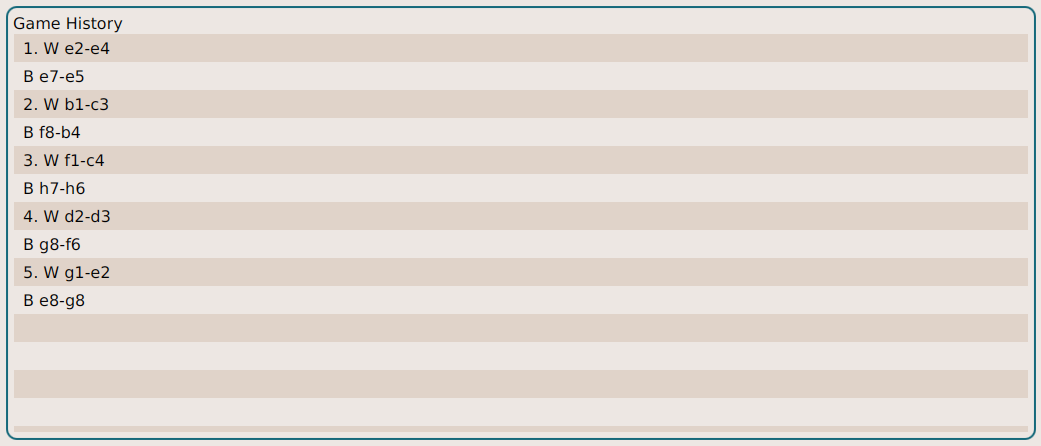
\includegraphics[width=\textwidth,height=5.0cm,keepaspectratio]{historique-coups}
\end{figure}

\subsection{Intelligence Artificielle} \label{AI}
\subsubsection{Heuristiques}
Afin de coder une bonne heuristique, aux échecs, il faut prendre en compte beaucoup d'éléments et revenir aux bases du jeu.
Notamment, il faut savoir ce qui importe dans une position, ce qui donne l'avantage ou ce qui assure une égalité. Essentiellement,
on se contente de vérifier certains points clés qui vont nous permettre d'émettre une évaluation sur une position.
Rappelons que le facteur de branchement aux échecs approche les 35.\\
Il y a de nombreux éléments à prendre en compte, et en voici certainement les plus impactants:
\begin{itemize}
    \item Le Matériel: chaque pièce (sauf peut-être le roi) possède une valeur. On va donc s'occuper de compter pour les 2 camps le "potentiel"
    dans une position. Plus on a de matériel (pièces donc), plus on a de chances d'avoir l'avantage, en particulier par un bon contrôle de l'échiquier.
    \item La sécurité du Roi: Le Roi est la pièce la plus importante aux échecs, et souvent, le joueur qui a un avantage est celui qui va
    avoir un Roi qui n'est pas en danger. Pour estimer cela, on peut en particulier vérifier le nombre de coups où l'on peut mettre le Roi en échec,
    combien de coups permettent de l'en sortir, et la fréquence des échecs. Plus un Roi est vulnérable, plus il y aura des possibilités
    de le mettre en échec.
    \item Le contrôle du centre: Aux échecs, le centre est un emplacement clé, puisqu'il peut donner un accès efficace à toutes les parties de
    l'échiquier. Généralement, obtenir un bon contrôle du centre est un facteur qui va jouer dans l'évaluation d'une position.
    \item L'activité: Si l'on a peu de coups légaux que l'on peut jouer, c'est très souvent parce que l'on est en position de désavantage. Cela peut
    signifier que l'on est forcé à jouer certains coups.
    \item La structure de pions: Plus on aura une structure de pions solide, plus on aura de potentiel d'attaque et de défense puisque les pions sont
    des pièces "faibles" lorsqu'ils sont seuls et/ou non défendus.
    \item La promotion: Plus on a de pions avancés, plus on a de chance d'atteindre la dernière rangée et changer notre pion en une pièce plus importante,
    comme la Dame par exemple, nous donnant plus d'options.\\
\end{itemize}

Seulement ceux-là sont cités ici, mais en réalité, il y a plus de 20 points clés nous permettant d'évaluer une position de manière efficace.
Enfin, afin d'obtenir une bonne heuristique aux échecs, il faut considérer tous ces points et faire une somme. C'est la marche à suivre puisque
il s'agit d'un jeu à somme nulle, c'est-à-dire que le gain d'un joueur correspond exactement à la perte de l'autre. En d'autres termes, si un joueur gagne (+1), l'autre perd (-1), et si la partie est nulle, aucun des deux joueurs ne gagne ni ne perd (0-0). \\
Dans ce projet, le groupe a développé une multitude d'heuristiques permettant d'évaluer des positions. Essentiellement, elles peuvent être regroupées
en deux catégories: Heuristiques "STANDARD" et Heuristiques "ENDGAME" ("Fin de partie"). En se servant du design pattern Composite, on combine les
heuristiques codées afin de se baser sur "beaucoup" de facteurs dans le but d'obtenir une évaluation d'une position la plus précise possible. Ainsi,
l'Intelligence Artificielle (MiniMax et AlphaBeta) utilise ces évaluations pour en déduire un "meilleur coup". STANDARD et ENDGAME sont les 
heuristiques par défaut lorsque l'IA est lancée. Le programme vérifie à tout moment (après chaque coup joué ou après chaque coup repris)
si le jeu se trouve être dans un stade de fin de partie ou non. Si la configuration est considérée être une fin de partie, alors l'heuristique utilisée
parl'IA devient ENDGAME, afin de prendre en compte des facteurs propres aux fins de partie. Autrement, elle utilise la STANDARD.\\
Voici quelques exemples d'heuristiques que le groupe a pu développer:
\begin{itemize}
    \item KingSafetyHeuristic : Une heuristique évaluant la sécurité du Roi.
    \item MaterialHeuristic : Une heuristique évaluant le matériel disponible de chaque côté.
    \item SpaceControlHeuristic : Une heuristique évaluant le contrôle de l'échiquier en se basant notamment sur le nombre
    de coups possibles.
    \item DevelopmentHeuristic : Une heuristique évaluant le développement des pièces sur l'échiquier.
    \item KingActivityHeuristic : Une heuristique évaluant l'activité du Roi (utilisée pour les fins de partie).
\end{itemize}

\subsubsection{Algorithmes}
Dans cette partie Intelligence Artificielle, on va essentiellement se servir des 3 algorithmes suivants (dont 2 vus au dernier semestre):
\begin{itemize}
    \item MiniMax: Visant à retourner l'option la plus adéquate dans une certaine position, on utilise des arbres pour savoir quelle branche va être la
    plus intéressante, que ce soit pour l'ami, comme pour l'ennemi. On est en O($b^d$) en temps, où b est le facteur de branchement et d la profondeur.
    En espace, c'est du O(d), soit le nombre de niveaux dans l'arbre pour une approche basée sur du DFS.
    \item AlphaBeta-pruning: Cet algorithme se repose sur MiniMax, mais peut permettre d'aller à une profondeur deux fois plus grande si les nœuds de
    l'arbre sont organisés du plus petit au plus grand. Ici, la valeur des nœuds va être une évaluation. La complexité en espace ne change pas, mais
    en temps nous sommes donc en O($b^p$) où p = d/2.
    \item MonteCarloTreeSearch:
    Celui-ci peut se décomposer en quatre étapes : \textbf{Selection}, \textbf{Expansion}, \textbf{Simulation}, et \textbf{BackPropagation}. Pour faire simple, on va choisir (Selection) des branches à explorer. Cela peut être les nœuds qui vont être impactants sur la recherche du meilleur coup, ou encore des nœuds qui n'ont pas encore été explorés. Il s'agit de l'UCT (Upper Confidence bound applied to Trees).\
    L'UCT est une formule permettant d'équilibrer l'exploration et l'exploitation dans la sélection des coups :
    \begin{equation}
    UCT = \frac{w(i)}{s(i)} + C \sqrt{\frac{\ln(N)}{s(i)}}
    \end{equation}
    où :
    \begin{itemize}
        \item $w(i)$ est le nombre de victoires du nœud $i$.
        \item $s(i)$ est le nombre total de simulations passées par ce nœud.
        \item $N$ est le nombre total de simulations effectuées depuis la racine de l'arbre.
        \item $C$ est un coefficient ajustable permettant de pondérer l'exploration.\
    \end{itemize} 

    L’UCT permet ainsi d’équilibrer l’exploration de nouveaux coups et l’exploitation des meilleurs coups déjà identifiés.
    Cela permet à l’algorithme MCTS de converger vers des coups optimaux tout en continuant à explorer de nouvelles options lorsque cela est nécessaire.
    Ensuite, après avoir choisi la branche, on se positionne à la feuille de cette branche,
    puis on simule un coup aléatoirement (Expansion) et on l'évalue. Maintenant, à partir de ce nouveau nœud, on simule une partie ou une pseudo-partie
    aléatoirement pour estimer le résultat potentiel. Finalement, lorsque l'on obtient un résultat, on fait remonter l'évaluation (BackPropagation)
    et/ou les informations importantes vers le haut de l'arbre pour plus tard agir en conséquence. En temps, on se rapproche de O(n*d), où n est le
    nombre de simulations effectuées, et d la profondeur moyenne. En espace, dans le pire des cas, on peut se trouver en O(N) où N est le nombre
    de simulations jouées. Maintenant, dans le cas moyen, on est en O($b^p$) avec d la profondeur et b le facteur de branchement.
    Cependant, dans le cadre de ce projet, MCTS n'est pas borné par une profondeur. On peut donc dire que l'on se trouve en O(N).\\
    En ce qui concerne la partie structures de données, le MCTS se base une classe Java, appelée dans le code 'TreeNodeMonteCarlo'.
    Comme son nom l'indique, il s'agit d'un objet représentant un noeud de l'arbre sur lequel l'algorithme va se dérouler.
    Essentiellement, cet objet va contenir les informations suivantes:
    \begin{itemize}
        \item GameState représentant la configuration de la partie
        \item Noeud parent (objet de même type)
        \item Noeuds enfants (objets de même type)
        \item Le nombre de victoires constatées depuis ce noeud
        \item Le nombre de visites de ce noeud (pour l'UCT et le winrate d'un coup)
        \item Le coup qui a amené à ce noeud depuis une configuration précédente
    \end{itemize}
    En reliant ces noeuds par des coups, on arrive à contruire un (pseudo-)arbre et à appliquer l'algorithme du Monte Carlo Tree Search dessus.
\end{itemize}

\par Notons que tous les algorithmes s'effectuent sur des arbres, et AlphaBeta ainsi que MiniMax se servent d'une heuristique pour évaluer chaque position.
PARLER DES OPTIMISATIONS D'IA MISES EN PLACES ET PEUT-ETRE CELLES ENVISAGÉES OU POSSIBLES;

\subsection{Zobrist hashing} \label{Zobrist}
Le Zobrist hashing est une fonction utilisée en particulier dans les jeux comme les échecs ou le Go, où le but est d'attribuer un codage "complexe" à
une position, pour éviter d'analyser une position plus d'une fois. Ainsi, on peut gagner en performance, notamment dans les algorithmes d'IA, où les
états de jeu peuvent se répéter un grand nombre de fois. On va se servir de ce qu'on appelle des "tables de transposition", qui sont des tables de
hachage indexées par une position. Dans notre cas, les positions sont encodées par 12 bitmaps et quelques booléens
supplémentaires pour les règles spécifiques.
\\Nous disposons des structures suivantes pour générer nos hash:\\
\begin{itemize}
    \item long PIECES[64][12]
    \item long EN\_PASSANT[8]
    \item long CASTLING[16]
    \item long SIDE\_TO\_MOVE
\end{itemize}

Nous générons donc au départ des nombres aléatoires pour chaque combinaison possible de case et de pièce, que nous mettons dans le tableau \textit{PIECES}.
Nous générons également des nombres correspondant aux en passant possibles ainsi qu'aux droits de roque. Il y a 8 configurations possible pour le en passant :
une pour chaque colonne ou un en passant pourrait être en cours.
Il y a 16 configurations possibles pour le roque, le petit et le grand roque de chaque couleur encore possible ou non (2 valeurs pour 4 roques différents soit 2**4).
Une fois ces nombres générés, on va pouvoir créer des hash correspondant à un état de plateau en faisant un XOR sur chaque pièce sur le plateau aisni que sur
les droits particuliers que nous avons pour le en passant et le roque. Il faut également XORer le joueur courant.
Ensuite, lorsqu'un mouvement est fait, il faut mettre à jour le hash, grace au XOR afin de corrrespondre au nouveau plateau de jeu.

Nous avons également implémeneté une version simplifiée du zobrist hashing, qui ne prend en compte que les pièces sur le plateau.

La version simplifiée est utilisée pour la règle du fifty move rule, où il ne faut pas revoir le même plateau 3 fois au cours d'une partie.
La version classique est très utile pour l'intelligence artificielle, pour le calcul des heuristiques en particulier, ce qui nous évite de reclaculer des heuristiques 
à partir du moment où on l'a calculée une fois. Le gain de temps est considérable en particulier lorsqu'on utilise des heuristiques lourdes à calculer.

\subsection{Cache}
Afin que le programme soit plus performant, nous avons mis en place un système de "cache". Ce dernier permet d'éviter de recalculer plusieurs fois la même valeur en stockant le résultat grâce au Zobrist hashing mentionné précédemment.\\


Nous avons pris la décision de stocker les valeurs les plus lourdes à calculer réutilisée par notre programme :
\begin{itemize}
    \item Boolean isCheckWhite : Un booléen activé si le roi blanc est attaqué (échec).
    \item Boolean isCheckMateWhite : Un booléen activé si le joueur blanc est échec et mat.
    \item Boolean isCheckBlack : Un booléen activé si le roi noir est attaqué (échec).
    \item Boolean isCheckMateBlack : Un booléen activé si le joueur noir est échec et mat.
    \item Boolean isStalemateWhite : Un booléen activé si le joueur blanc est en situation de pat.
    \item Boolean isStalemateBlack : Un booléen activé si le joueur noir est en situation de pat.
    \item Long whiteAttackBitboard : Un long utilisé comme bitboard représentant les cases attaquées par les pièces blanches.
    \item Long blackAttackBitboard : Un long utilisé comme bitboard représentant les cases attaquées par les pièces noires.\\
\end{itemize}

L'utilisation de types élémentaires aurait été une solution pour économiser de l'espace, en utilisant le conteneur Optional présent en Java, néanmoins la nécessité du gain de temps nous oriente vers l'implémentation actuelle, des allocations fréquentes de Optional pouvant ralentir le programme lors de son execution.

\subsection{Bidirectional Map}
COMPLETER.

\subsection{Iterative Deepening}

L'algorithme d'approfondissement itératif est utilisé dans notre projet en appui de l'algorithme AlphaBeta et de sa version parallèle. Il réalise des recherches en augmentant progressivement la profondeur (1, 2, 3, etc.) de manière successive. À chaque itération, le meilleur coup trouvé est placé au début de l'arbre de recherche, améliorant l'ordonnancement des coups pour l'algorithme d'élagage. Ainsi, ce procédé permet de réduire considérablement le nombre de positions évaluées.\\

Le véritable avantage de l'approfondissement itératif vient de sa capacité à fournir une solution en temps réel tout en affinant progressivement l'analyse du jeu, optimisant ainsi le processus de décision dans le cas d'une limite de temps appliquée au joueur IA.
Dans le cadre d'un jeu comme les échecs, il permet également de gagner du temps via l'amélioration de l'élagage.

\subsection{Code propre}
Nous avons effectué plusieurs refactor afin d'arriver à une architecture plus claire au cours du projet. Dans les dernières semaines de développement, 
lorsqu'il y avait moins de nouvelles features ajoutées, nous nous sommes penchés sur les outils de qualité de code tels que \textit{Checkstyle} ou \textit{PMD}.

Nous avons commencé par rajouter de la documentation sur les classes ainsi que sur leurs fields et méthodes. 
Le mot clé final a été ajouté sur les variables et fields le nécéssitant. Cela permet de rajouter de la sécurité ainsi que la lisibilité du code.
Les noms de fonctions ainsi que de variables on été modifiés afin de suivre les normes. Nous avons également suprimé la quasi totalité des \textit{System.out/err}.

Après avoir corrigé de nombreux warnings, environ 500 d'entre eux sont toujours présents.
Les règles utilisées dans PMD sont disponibles dans le fichier \textit{pmd-rules.xml}.
Certains de ces warnings ont été jugés 
comme peu utile comme par exemple les logs devant être entourés de barrières (ce qui est fait dans nos méthodes de logging) ou la taille des commentaires,
qui correspondait au style Google mais pas à celui de PMD. 
Ayant décidé d'avoir une application multithreadée ( Bag of commands, vue, IA parralèle), nous avons décicé d'ignorer le warning interdisant l'utilisation de threads.
En effet, cela concerne les application utilisant Java Enterprise Edition, ce que nous ne faisons pas.
Le fait d'avoi au minium un constructeur par classe est également jugé inutile, en effet le compilateur le rajoute automatiquement s'il s'agit d'un constructeur vide.
Le fait de pouvoir faire un return anticpé dans une fonction est quasi nécéssaire, si nous ne voulons pas entourer le code dans 
d'énormes blocs de \textit{if}, nous avons donc supprimé la règle correspondante.
Certaines variables sont jugées trop courtes, mais dans certains cas, une variable courte est toujurs explicite (comme \textit{x} pour une position). 
D'autres sont trop longues, mais avec la présence d'autocomplétion dans la plupart des IDE, nous avons préféré garder des noms explicites, qui peuvent être compliqué à raccoucir,
comme \textit{isLastMoveDoublePush}.

Après avoir utilisé ces outils de clean code, nous sommes passés de plus de 6000 warnings à moins de 500.

\section{Architecture du projet}
Nous avons décidé de présenter le projet sous une forme d'architecture MVC personnalisée. Cette architecture est particulièrement pratique pour nous, développeurs, aussi bien en termes de maintenance que d'extensibilité.
Le Controller, ou plutôt le Bag Of Commands agit comme interprète entre la vue et le Model, il va recevoir des commandes de la part de la Vue et appeler les fonctions correspondantes dans le Model.
La vue a tout de même accès au Model, afin de récuperer les changements à afficher, ce qui évite de surcharcher le controller.

\begin{center}
    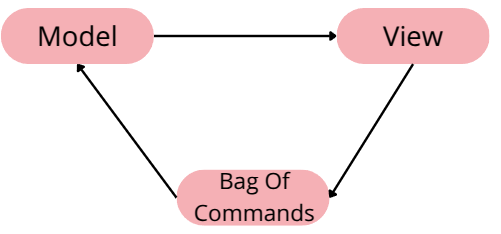
\includegraphics[width=0.5\textwidth]{MVC}
\end{center}

\subsubsection{Description des Modules}

\begin{itemize}
    \item \textbf{Model} : Gère la logique métier du jeu, incluant l'état de la partie, les règles d'échecs et les fonctionnalités comme l'historique et le timer, et même l'Intelligence Artificielle.
    \item \textbf{Controller} : Sert d'intermédiaire entre la Vue et le Model. Il gère les événements utilisateurs et orchestre les interactions entre les différentes couches.
    \item \textbf{Vue} : Responsable de l'affichage et des interactions avec l'utilisateur, qu'il s'agisse d'une interface CLI ou graphique.
    \item \textbf{Events} : Implémente un système d'observateurs pour gérer les notifications et la communication asynchrone entre les modules.
    \item \textbf{Utils} : Contient des outils génériques comme le gestionnaire de textes internationalisés (\texttt{TextGetter}) et les algorithmes d'intelligence artificielle pour le jeu.
    \item \textbf{Exceptions} : Contient les types d'exceptions personnalisées qui peuvent survenir dans le programme et nous permettant d'agir en conséquence.
\end{itemize}

\subsubsection{Model}
Le Modèle est lui même composé de plusieurs packages, afin de séparer les différentes patie de l'application :

\begin{itemize}
    \item \textbf{AI} : Contient toute la partie IA, soit le solver, les algorithmes et les heuristiques.
    \item \textbf{Board} : 
    \item \textbf{History} : Structure représentant l'historique de la partie sous forme de liste doublement chainée.
    \item \textbf{Parsers} : Parsing des fichers de configuration et de sauvegarde.
    \item \textbf{Piece} : 
    \item \textbf{Savers} : Sauvegarde des fchiers de jeu et de configuration.
\end{itemize}

\subsubsection{View}


\subsubsection{Controller}

\begin{center}
    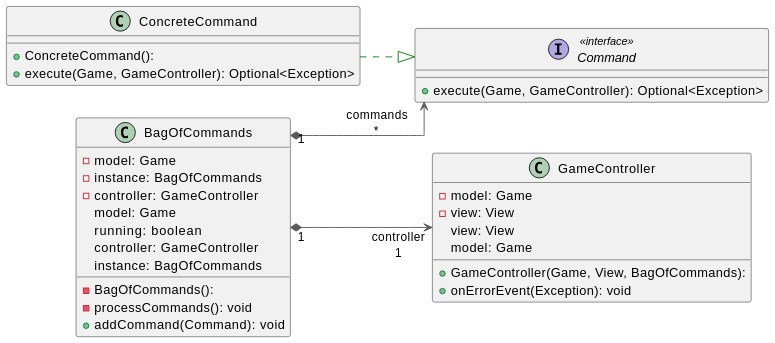
\includegraphics[height=\textwidth]{uml_controller}
\end{center}

\subsubsection{Design Patterns Utilisés}

Les différents design patterns utilisés dans ce projet sont les suivants : 
\begin{itemize}
    \item \textbf{Singleton} : Utilisé pour la classe \texttt{Game} pour s'assurer qu'une seule instance de la partie est présente.
    La classe \texttt{BagOfCommands} utilise ce design pattern afin que la gestion des commandes ne soit gérée que par un seul bag.
    \item \textbf{MVC} : L'architecture principale du projet, séparant clairement la logique métier, l'affichage et la gestion des événements. C'est un MVC modifié,
 grâce au design pattern Observer qui va permettre d'envoyer des messages du Model vers la Vue. Cela permet notamment une meilleur flexibilité dans la
 gestion d'évènements.
    \item \textbf{Observer} : Permet de notifier la Vue des modifications dans le Model.
    \item \textbf{Command} : Utilisé pour simplifier le Controller. Chaque commande a un objectif précis, effectuer un certain traitement dans le Model.
    \item \textbf{Bag of Commands} : Utilisé pour gérer les Commandes. Nous pourrons gérer l'ajout de plusieurs commandes en parallèle.
    \item \textbf{Composite} : Utilisé pour combiner les heuristiques qui sont manipulées par l'Intelligence Artificielle.
    \item \textbf{Prototype} : Utilisé avec la fonction getCopy() qui génère un clone de la classe demandée.
\end{itemize}


\section{Performances et Limitations}
\subsection{Traces}
Pour exprimer les performances de notre programme et plus généralement pour pouvoir comparer des version différentes, nous avons réalisé plusieurs
traces à l'aide de \textit{Intellij Profiler}. À l'aide de ce logiciel, il est possible de réaliser des traces comportant le temps d'exécution, l'occupation des threads
ou encore la mémoire utilisée par notre programme à tout instant comme le présente la figure \ref{trace_ex}.

\begin{figure}[h]
    \centering
    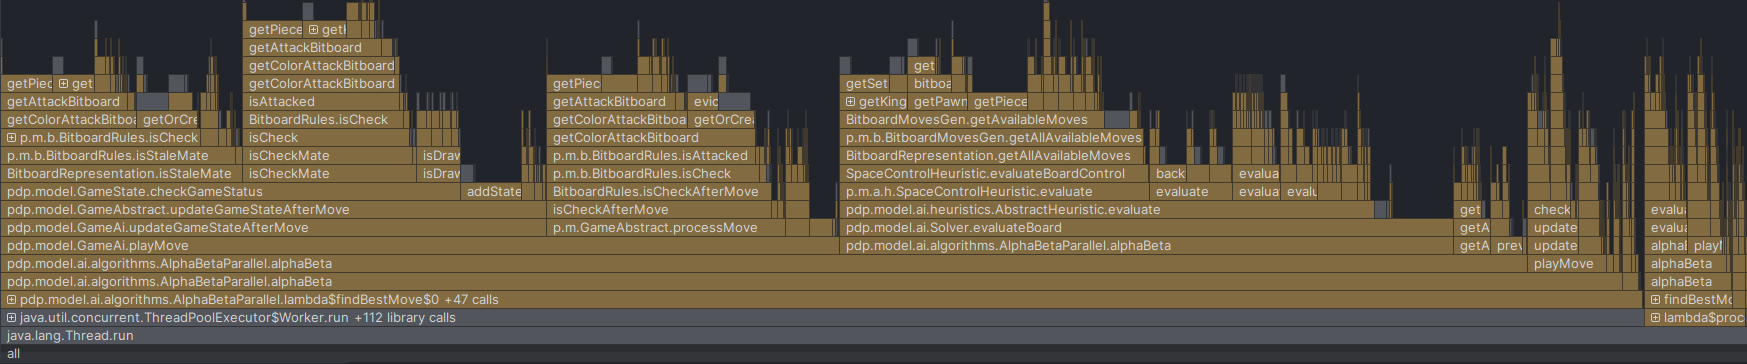
\includegraphics[width=\textwidth,height=6.0cm,keepaspectratio]{trace_example.png}
    \caption{Exemple de trace d'exécution pour visualiser le temps d'exécution découpé par fonctions}
    \label{trace_ex}
\end{figure}

Dans cette représentation il est possible de voir clairement quelles sont les fonctions les plus chronophages mais il est également possible 
de comparer deux traces afin de voir les différences de performances entre plusieurs versions, algorithmes ou heuristiques \ref{trace_ex2}.

\begin{figure}[h]
    \centering
    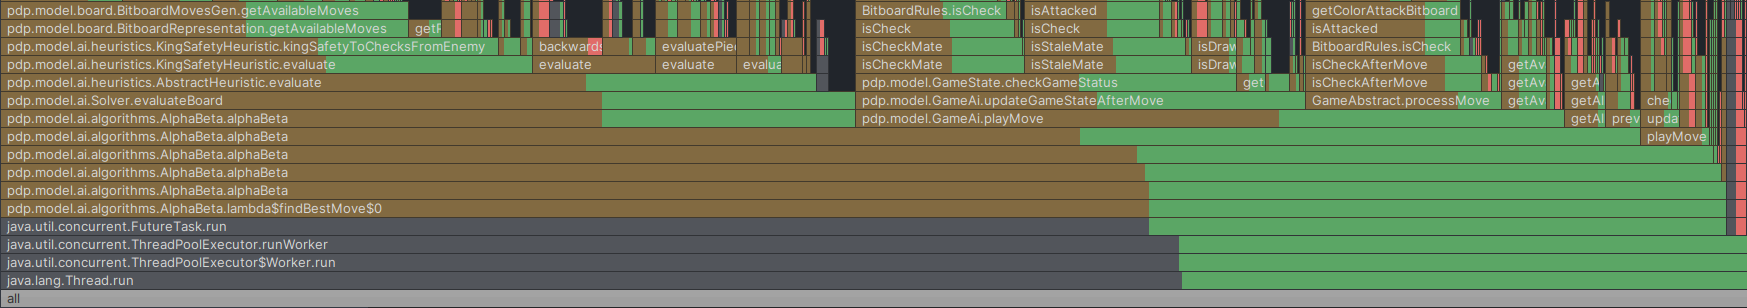
\includegraphics[width=\textwidth,height=6.0cm,keepaspectratio]{trace_ex2.png}
    \caption{Exemple de comparaison entre deux traces d'exécution}
    \label{trace_ex2}
\end{figure}

Dans ce graphique on superpose donc deux traces afin de pouvoir analyser le temps gagné ou perdu pour chaque fonction. Il faut donc définir une trace référente, et les temps
s'afficheront en fonction de celle-ci. Tous les rectangles verts signifient que l'on gagne du temps par rapport à l'autre exécution tandis que les rectangles rouges représentent
les endroits où l'exécution référente est plus lente. Des informations supplémentaires sont également disponibles notammement pour afficher les temps gagnés/perdus en pourcentage
que nous utiliserons pour donner des gains/pertes chiffrés.

Enfin il est possible d'obtenir une vue comme le présente la figure \ref{thread_ex} afin de voir l'état des différents threads de la machine (running, sleeping). Ici, chaque thread est représenté
par une ligne, et on peut lire sont état au fil du temps de l'exécution à l'horizontal. Dans ces graphiques les rectangles verts
représentent lorsque le threads est actif, il sont rouges lorsque qu'il sont endormis. Il permet donc de voir l'équilibre des charges et si la parallélisation est réellement efficace.
Nous utiliserons donc ce graphe pour vérifier le caractère parallèle de certaines optimisations.

\begin{figure}[h]
    \centering
    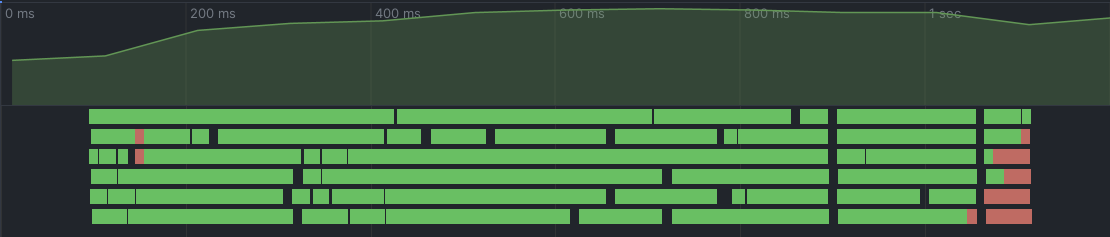
\includegraphics[width=\textwidth,height=6.0cm,keepaspectratio]{threads_ex.png}
    \caption{}
    \label{thread_ex}
\end{figure}

\subsection{Optimisations Intelligence Artificielle}
À la suite de l'implémentation des algorithmes d'IA démandés, nous avons remarqué que les performances du programmes étaient assez contrastées. En effet, le facteur
de branchement moyen étant 35, le passage d'une profondeur à une profondeur+1 demande un temps de calcul beaucoup plus long. Nous avons donc pu atteindre la profondeur 3
en temps raisonnable sans optimisation. Afin d'améliorer l'IA nous avons donc ensuite mis en place différentes optimisations. Pour commencer nous avons adapté nos heuristiques
pour qu'elle puissent utiliser directement les bitboard afin de tirer le meilleur de la structure de données et d'enlever des couches d'abstractions. Nous avons par la suite 
remarqué que le calcul de certaines fonctions était chronophage et ne pouvaient pas être diminué en complexité facilement. C'est par exemple le cas des fonction de détection de 
l'échec, échec et mat, pat qui sont utilisé lors de l'évaluation du plateau mais également lorsque qu'un coup est jouer pour vérifier si le coup est légal (sans compter le fait 
qu'un plateau peut apparaître plusieurs fois). Grace au Zobrist hashing, nous avons donc implémenté une sorte de cache pour ne pas reclaculer ces fonctions pour le même plateau 
plusieurs fois. Nous avons donc stocké les résultats des fonctions précédentes ainsi que les bitboards de mouvements puisqu'elles sont très solicitées lors de l'évaluation des
plateaux. Nous avons donc pu comparer une exécution avec un cache de 10000 entré et une autre sans cache comme le présente la figure \ref{cache_cmp}.

\begin{figure}[h]
    \centering
    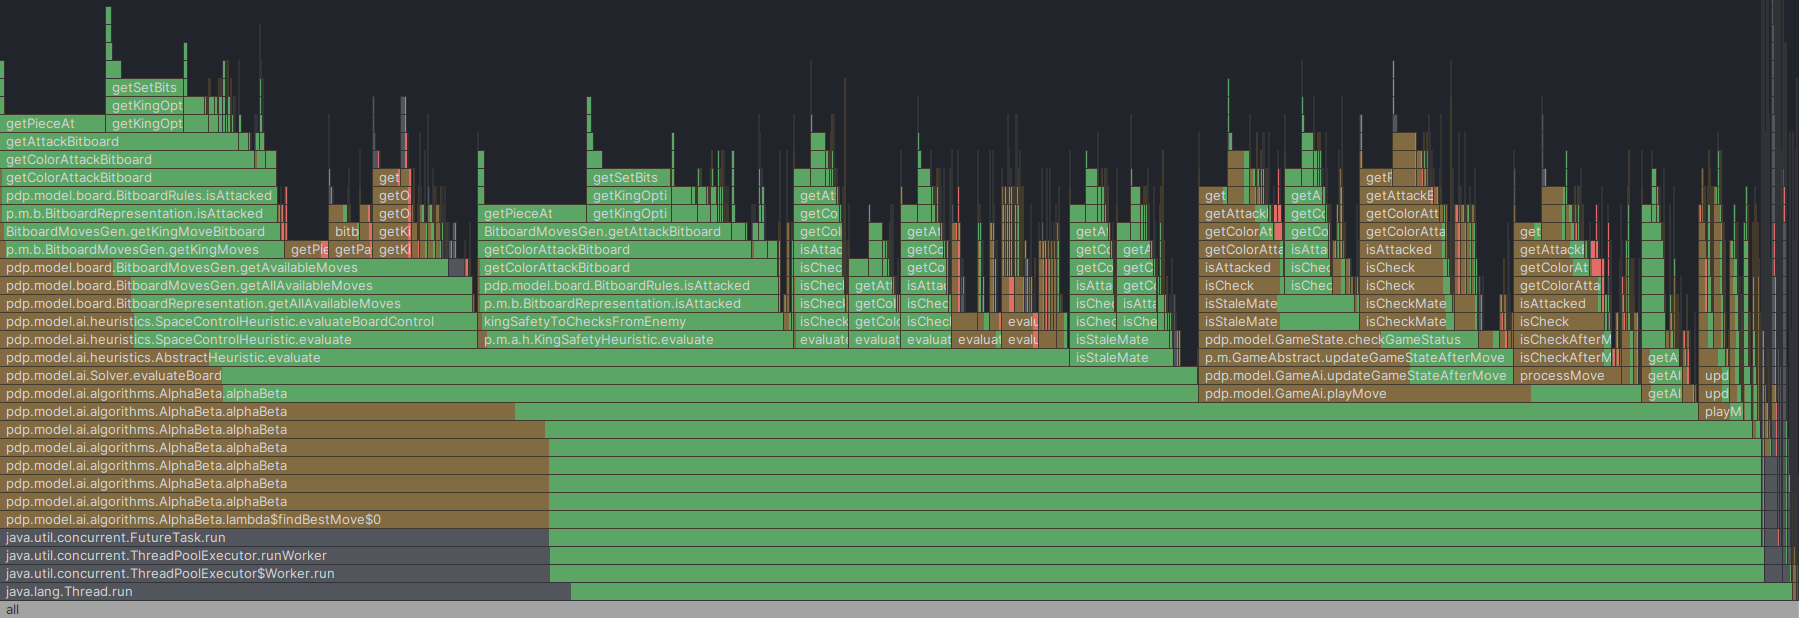
\includegraphics[width=\textwidth,height=6.0cm,keepaspectratio]{cache_compare.png}
    \caption{Comparaison des traces d'exécutions avec et sans cache}
    \label{cache_cmp}
\end{figure}

Sur cette trace on remarque un gain temps de l'ordre de 68\% lorsque l'on utilise un cache. Globalement, nous gagnons du temps car il n'y a plus de calculs couteux
effectués plusieurs fois. Puisque toutes ces fonctions sont calculées afin de pouvoir jouer le coup (car il faut vérifier que le coup ne met pas fin à la partie et 
est bien légal), la grande différence se fait dans lors de l'évaluation car on économise ici près de 80\% du temps nécessaire sans cache. Mais si cela est moins significatif,
celui-ci permet de gagner environ 25\% de performance sur la fonction \textit{playMove} car il était obligatoire de vérifier deux fois la mise en échec lorsque qu'un coup était joué,
une première pour vérifier que le roi n'était pas en échec ainsi que pour vérifier que la partie n'avait pas atteint une situation de pat
COMPARAISON ALPHA\_BETA, ALPHA\_BETA\_PARALLEL, ALPHA\_BETA\_IT

\subsection{Profondeur de recherche}
d = 6+ très long.

\subsection{Vue}
JavaFX, bien que pratique pour développer des GUI en Java, présente des limites en termes de performance, en particulier en ce qui concerne
la fluidité et les animations. En effectuant quelques recherches, on se rend compte que l'engine de rendu du framework repose principalement
sur Java2D et utilise une pipeline GPU limitée, ce qui peut causer des ralentissements, surtout pour les logiciels nécessitant du refresh
fréquent. Java est globalement un langage rapide, mais il est limité. Si le projet avait été développé en C++, avec notamment
l'aide d'OpenGL, la vue serait bien plus efficace. Sinon, en comparaison, l'utilisation d'un engine dédié comme Unity ou Godot permettrait
un meilleur rendu général, tandis qu'une approche basée sur les technologies web (HTML, CSS, WebGL) offrirait une
optimisation native des performances. Finalement, JavaFx se trouve être une solution pour l'interface graphique dans notre cas, et même si
pratique et bien architecturé, reste limité en termes de performances graphiques.

\section{Critiques et Perspectives}
Ce projet a été décomposé en une soixantaine de besoins afin d'être réalisé. Même si cette réalisation a été plutôt atteignaible, il est important de
faire part des points faibles de l'application, de ses points forts, et potentiellement des nouvelles fonctionnalités ou améliorations qui pourraient ou 
auraient pu voir le jour dans le cadre de cette U.E.
\subsection{Critiques Négatives}
\subsubsection{MonteCarloTreeSearch}
Le Monte Carlo Tree Search (MCTS) est largement utilisé dans les jeux de stratégie tels que le Go, où la non-présence d'heuristiques efficaces rend les méthodes classiques d'IA comme AlphaBeta moins adaptées. Cependant, aux échecs, MCTS est rarement employé à cause d'une multitude de limitations.
Premièrement, les échecs bénéficient d'évaluations positionnelles efficaces et d'une base théorique bien établie, ce qui permet aux algorithmes classiques comme Minimax avec AlphaBeta d'explorer l'arbre de jeu de manière plus efficace. Contrairement à des derniers, MCTS ne se base pas sur des critères d'évaluation et d'optimisations. Ensuite, MCTS est intrinsèquement plus lent que les méthodes basées sur Minimax. En effet, sans optimisation spécifique, il doit effectuer un grand nombre de simulations pour obtenir une estimation intéressante de la valeur d'un GameState. Dans un jeu comme les échecs, où le facteur de branchement moyen est élevé, MCTS a besoin d'un (très) grand nombre d'itérations pour converger vers des décisions "optimales" comparables à celles d'Alpha-Beta Pruning. La simulation de coups est très "Brute-Force", surtout sans optimisation, car le choix des coups par l'algorithme s'effectue de manière complètement aléatoire (pour la partie simulations).
Enfin, les engines d'échecs modernes tirent parti d'optimisations telles que le move ordering, des bibliothèques d'ouvertures, améliorant ainsi les performances d'Alpha-Beta Pruning. Bien que le MCTS puisse être optimisé par des techniques spécifiques d'IA comme les réseaux de neuronnes, son efficacité brute sans ces améliorations reste inférieure aux méthodes classiques pour les échecs. Maintenant, le groupe admet que son implémentation du MCTS est 
lente de base, notamment à cause d'un grand nombre de deep copies d'objets GameState
Ainsi, bien que MCTS soit une approche puissante pour certains jeux, son application aux échecs reste limitée en raison de sa lenteur et de son inefficacité sans optimisation.

\subsubsection{Clean Code}
Même en enlevant les règles nous paraissant superflues, nous avons toujours environ 500 warning à résoudre.
Afin de retirer les \textit{System.out/err}, nous avons crée des fonctions \textit{print} et \textit{error}, qui sont des wrappers de ces fonctions. Il serait plus judicieux de créer
des loggers pour ces opérations.
Certaines classes possèdent trop de méthodes, elles sont qualifiées de \textit{God Class}. Il serait nécessaire de faire un refactor total du projet, ce quicorrespond à un projet à part entière.
Il en est de même pour les méthodes trop complexes, qu'il faudrait découper en sous parties.
\subsection{Critiques positives}
COMPLETER ICI PAR DES CRITIQUES POSITIVES.
Par exemple, la communication entre IA (avec stockfish etc.).

\subsection{Perspectives}
\subsubsection{Mode Multi-joueur}
Certainement l'amélioration la plus intéressante serait un mode multi-joueur, dans le même style que chess.com ou lichess.org pour ne citer qu'eux.
Le projet prendrait néanmoins une toute autre direction puisque les joueurs devraient se connecter à un serveur afin de jouer en temps réel. Une
autre solution serait le Peer-To-Peer.

\subsubsection{Tourner l'échiquier}
Dans notre application, c'est toujours les pièces blanches qui sont situées en bas. Une amélioration graphique serait la possibilité d'inverser le plateau
de jeu en pleine partie de telle sorte que les pièces noires seraient en bas. Cela deviendrait plus pratique pour les utilisateurs qui jouent les Noirs.

\subsubsection{Coups préparés}
Lorsque le joueur joue contre une IA, il pourrait effectuer un 'pre-move', c'est-à-dire préparer un coup sur l'échiquier avant que l'IA n'ait joué. Dès que 
le joueur IA jouerait son coup, le coup préparé par l'utilisateur serait immédiatement joué. Ceci peut être pratique en début de partie ou en fin de partie 
ou plus souvent lorsqu'il n'y a pas nécessité de réflexion pendant longtemps.

\subsubsection{Analyser des parties}
Une fonctionnalité supplémentaire pourrait concerner la Game Review. L'utilisateur serait capable à la fin d'une partie (ou lancer depuis un fichier en mode 
analyse) de se balader dans la partie, dérouler les coups notamment pour voir les erreurs ou les brillances qu'un joueur aurait faites.

\subsubsection{Surligner des coups}
L'utilisateur aurait la possibilité de "surligner" des coups afin de montrer des déroulements de partie ou d'y voir plus clair dans sa réflexion.
Cela ressemblerait à quelque chose du style :\\
\begin{figure}[h]
    \caption{Exemple surlignage de coups}
    \centering
    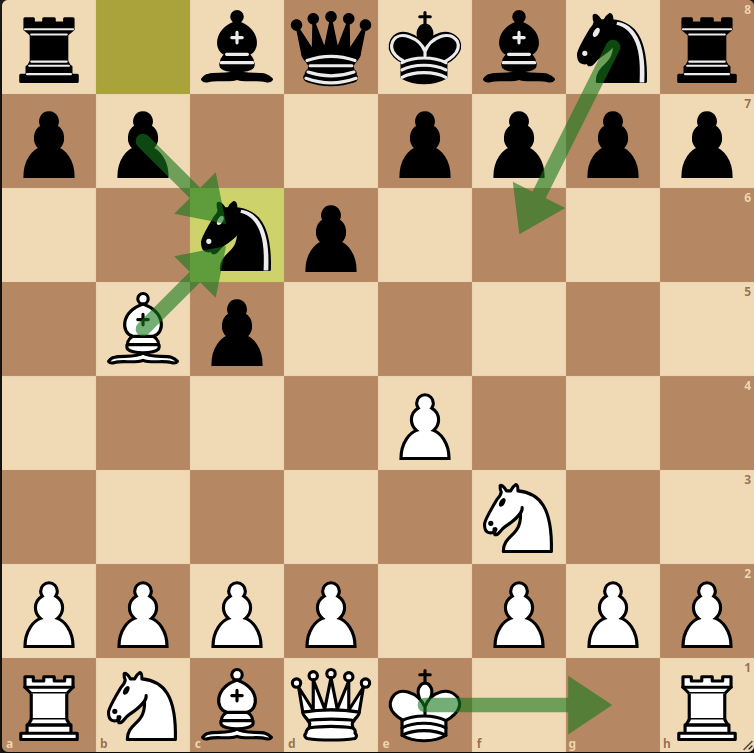
\includegraphics[width=\textwidth,height=6.0cm,keepaspectratio]{surlignage-coups}
\end{figure}


\section{Bibliographie}
 \bibliographystyle{plain}
 \bibliography{references}


\section{Besoins réalisés - Annexe}
\label{Spec}

Voici la liste exhaustive des besoins qui ont été réalisés lors de ce projet. Pour chaque besoin, on retrouve un code couleur représentant
son état de validation. Vert signifie validé, orange semi-validé, rouge non validé. Si ambiguïté ou besoin de détails il y a, une explication
est fournie afin d'éclaircir les choses. Parfois, le besoin peut être compris d'une autre manière. Nous rappelons qu'il s'agit de notre point de vue.
Un besoin que le groupe considère validé peut ne pas l'être pour d'autres, mais en tout état de cause, le but n'est pas de tricher.

\begin{longtable}{|c|p{5cm}|c|p{5cm}|}
    \hline
    \textbf{\#} & \textbf{Nom du besoin} & \textbf{Statut} & \textbf{Explication si ambiguïté} \\
    \hline
    \endfirsthead

    \hline
    \textbf{\#} & \textbf{Nom du besoin} & \textbf{Statut} & \textbf{Explication si ambiguïté} \\
    \hline
    \endhead

    \hline
    1 & Langage de programmation & \valid & \\
    \hline
    2 & Style de codage & \valid & \\
    \hline
    3 & Langue par défaut dans le code & \valid & \\
    \hline
    4 & Système cible & \valid & \\
    \hline
    5 & Documentation & \semivalid & COMPLETER SI BESOIN \\
    \hline
    6 & Tests & \valid & \\
    \hline
    7 & Bugs & \valid & \\
    \hline
    8 & Performances & \nonvalid & COMPLETER SI BESOIN \\
    \hline
    9 & Build-system & \valid & \\
    \hline
    10 & Frameworks de test & \valid & TestFX a été utilisé pour tester l'interface graphique. \\
    \hline
    11 & Gestion des options & \valid & \\
    \hline
    12 & Bibliothèque graphique & \valid & \\
    \hline
    13 & Internationalisation & \valid & \\
    \hline
    14 & Nom de l’exécutable principal & \semivalid & \\
    \hline
    15 & Usage général & \semivalid & COMPLETER SI BESOIN \\
    \hline
    16 & Aide en ligne de commande & \valid & \\
    \hline
    17 & Version & \valid & \\
    \hline
    18 & Mode verbose & \valid & \\
    \hline
    19 & Mode debug & \valid & \\
    \hline
    20 & Mode Blitz & \valid & Le temps de chaque joueur est donné à tout instant. Chaque joueur a un temps pour chaque coup, et non pour toute la partie afin de suivre la spécification (ce comportement ne correspond pas à la règle officielle du blitz). Affichage du temps restant après chaque coup.\\
    \hline
    21 & Durée du Blitz & \valid & \\
    \hline
    22 & Mode Contest & \valid & La partie est sauvegardée dans le fichier une fois le coup joué et affiché.\\
    \hline
    23 & Mode IA & \valid & \\
    \hline
    24 & Interface en ligne de commande & \valid & \\
    \hline
    25 & Interface graphique & \valid & \\
    \hline
    26 & Affichage de l'échiquier & \valid & Le temps affiché est le temps restant au joueur au moment du coup.\\
    \hline
    27 & Notation des coups & \valid & \\
    \hline
    28 & Représentation de l'historique & \valid & \\
    \hline
    29 & En passant & \valid & \\
    \hline
    30 & Roque & \valid & \\
    \hline
    31 & Promotion du pion & \valid & \\
    \hline
    32 & Abandon & \valid & \\
    \hline
    33 & Affichage des messages & \valid & \\
    \hline
    34 & Quitter et sauvegarder une partie & \valid & \\
    \hline
    35 & Sauvegarde de l’historique & \valid & L'historique est sauvegardé à la suite du plateau de jeu. \\
    \hline
    36 & Naviguer dans l'historique & \valid & \\
    \hline
    37 & Recommencer une partie & \valid & \\
    \hline
    38 & Fin de partie & \valid & \\
    \hline
    39 & Rejouer une partie & \valid & \\
    \hline
    40 & Format de fichier simplifié & \valid & L'historique est sauvegardé uniquement si le fichier d'origine contient un historique ou que la partie a été jouée depuis le début. Le format proposé étant ambigu (roques, en passant, etc), nous avons décidé d'ajouter un header au format FEN. \\
    \hline
    41 & Format de l'historique & \valid & Si un historique est fourni, la partie est chargée depuis ce dernier, sinon elle est chargée depuis le plateau de jeu. \\
    \hline
    42 & Fichier de configuration & \valid & \\
    \hline
    43 & Plateau de jeu & \valid & \\
    \hline
    44 & Module bitboard & \valid & \\
    \hline
    45 & État du jeu & \valid & L'historique est stocké dans la classe Game plutôt que GameState (choix d'implémentation).
    Game et GameState forment une structure contenant le joueur courant, le plateau, le temps (blitz) et l'historique.\\
    \hline
    46 & Fonctions de base GUI & \valid & \\
    \hline
    47 & Menu 'File' & \valid & \\
    \hline
    48 & Menu 'Game' & \valid & \\
    \hline
    49 & Menu 'About' & \valid & \\
    \hline
    50 & Affichage d'une partie en cours & \valid & \\
    \hline
    51 & Affichage des coups joués & \valid & \\
    \hline
    52 & Configuration d'une nouvelle partie & \valid & \\
    \hline
    53 & Heuristique d'évaluation & \valid & \\
    \hline
    54 & Algorithme Minimax & \valid & \\
    \hline
    55 & AlphaBeta-pruning & \valid & En plus de la version classique, une version Iterative Deepening a été implémentée. Les deux versions possèdent également une alternative parallèle (avec la moitié des threads disponibles sur la machine). \\
    \hline
    56 & Monte Carlo Tree Search & \valid & L'option --ai-simulations permet de paramétrer le nombre de simulations effectuées par l'IA. \\
    \hline
    57 & Profondeur de recherche & \valid & L'option n'est pas disponible pour l'algorithme MCTS. \\
    \hline
    58 & Choix des heuristiques & \valid & \\
    \hline
    59 & Heuristiques de fin de partie & \valid & L'heuristique ENDGAME a été prévue pour la fin de partie, et le solver change automatiquement l'heuristique utilisée en fonction de l'état du plateau. L'option --ai-endgame permet également de choisir l'heuristique de fin de partie utilisée. \\
    \hline
    60 & Temps de réflexion IA & \valid & Le temps de l'IA est borné uniquement lorsque l'option est présente. Cependant, les algorithmes possèdent toujours une profondeur de recherche et s'arrêtent lorsque l'une des bornes est atteinte (pour utiliser uniquement le temps, il faut utiliser une profondeur très élevée). \\
    \hline
\end{longtable}

Voici aussi une liste présentant les besoins "bonus", qui n'étaient pas présents dans la liste des besoins du cahier des charges.

\begin{needbox}[F61: Historique scrollable et cliquable]
    L'historique en GUI est scrollable, de telle manière que les coups sont lisibles même si la partie
    comporte un grand nombre de coups. Il est également possible de double-cliquer sur un coup pour revenir à celui ci si les deux joueurs sont d'accord.
\end{needbox}

\begin{needbox}[F62: IA paramétrable]
   Toutes les options d'IA, mis à part --ai-time, sont paramétrables en fonction de la couleur, en rajoutant 
   -b ou -w au nom de l'option. Par exemple --ai-mode-w.
\end{needbox}

\begin{needbox}[F63: Algorithmes d'IA supplémentaires]
   Une version Iterative Deepening est disponible. Elle permet une meilleure précision lorsque l'option time est activée. Cet algorithme est également plus performant que l'AlphaBeta classique.
   Des versions parallélisées des algoritmes d'AlphaBeta et AlphaBeta Iterative Deepening sont aussi disponibles.
\end{needbox}

\begin{needbox}[F64: Header FEN]
   Afin d'éviter toute ambiguité lors de chargement de partie depuis un fichier, nous prenons en charge un header au format FEN. Cela permet de conserver les droits de roque, d'en passant et la fifty move rule à jour.
\end{needbox}

\begin{needbox}[F65: Thèmes GUI]
    Différents thèmes sont disponibles dans le menu Options du GUI. Il est également possible de créer et sauvegarder ses propres thèmes.
\end{needbox}

\begin{needbox}[F66: Monitoring de l'IA]
    Il est possible de suivre les performances de l'IA dans le GUI. En activant l'option Monitor dans le menu Options, celui ci permet d'observer le nombre de noeuds, le temps de recherche, le nombre de noeuds visités par senconde pour chaque coup ainsi que les valeurs moyennes au cours de la partie..
\end{needbox}

\begin{needbox}[F67: Mode UCI]
    Afin de pouvoir communiquer avec d'autres chess engines, notre programme intègre une version minimale de la norme UCI. Il est possible de réaliser des parties contre Stockfish à l'aide de scripts externes.
\end{needbox}

\begin{needbox}[F68: Heuristique à poids]
    Il est possible de configurer l'heuristique Standard en lui ajoutant des poids personnalisés (float), via l'option --ai-weight-b ou --ai-weight-w afin d'améliorer la précision de l'heuristique.
\end{needbox}


\end{document}